\documentclass[edipack_sp.tex]{subfiles}
\begin{document}

\section{Examples}\label{SecExamples}
In this section we illustrate and benchmark the functionalities and of  \NAME
library and its interfaces as a solver for DMFT through a variety of examples. We also discuss in detail the relevant code parts from different programming languages. 
The codes, the data and the scripts to rework some of the examples presented here, as well as additional upcoming tutorials, can be found in the repository \href{https://github.com/EDIpack/EDIpack2examples}{github.com/EDIpack/EDIpack2examples}.  

Some tasks---particularly those associated with the implementation of the DMFT self-consistency---are inherently independent of \NAME itself, and the impurity solver is agnostic about them. 
Thus, in the implementations using Fortran, Python or other \NAME interfaces to scientific toolboxes, we adopt a reverse communication strategy, which requires the user to independently carry out these parts or, equivalently, to take advantage of existing utilities. 

In our examples based on the Fortran APIs, we rely on external open-source libraries, such as DMFTtools (see \href{https://github.com/aamaricci/DMFTtools}{github.com/aamaricci/DMFTtools}), to perform specific tasks, including evaluating the local Green’s function, implementing the self-consistency, constructing the tight-binding model, or calculating the kinetic energy.
Where appropriate, we include comments that reference these external procedures.

On the other hand, the results obtained with w2dynamics rely on the internal framework provided by the software itself -- see the script \texttt{DMFT.py} \cite{Wallerberger2019CPC}, which seamlessly handles all these tasks.
Similarly, the TRIQS library offers a comprehensive framework for manipulating Green’s functions and related quantities \cite{Parcollet2015CPC}, making these tasks easily accessible while maintaining very high standards of optimization and accuracy.


\subsection{Hubbard model on the Bethe lattice (Fortran/C++ API, {\tt ed\_mode=normal})}\label{SecExamplesBetheDMFT}
The description of the Mott transition using the Hubbard model on the Bethe lattice is conventionally regarded as the standard test bed for any DMFT implementation.  \cite{Georges1996RMP,Rozenberg1999PRL,Kotliar1999EPJB,Kotliar2000PRL,Kotliar2002PRL}.
%
Here, we present a guided implementation of the DMFT 
solution for the Bethe lattice at $T=0$ using \NAME as impurity
solver.
The model under consideration is the Fermi-Hubbard Hamiltonian:
$$
H = -t \sum_{\langle ij\rangle,\s} c^\dagger_{i\s} c_{j\s} + 
    U \sum_i n_{i\up}n_{i\dw},
$$
where $c^\dagger_{i\s}$ ($c_{i\s}$) are the creation (annihilation) 
operators for an electron at site $i$ with spin $\s$, and 
$n_{i\s} = c^\dagger_{i\s} c_{i\s}$ is the corresponding occupation 
operator. The first sum runs over nearest-neighbor pairs
$\langle ij \rangle$.
We consider the system defined on a Bethe lattice with density of states
$\rho(\e)=\frac{2}{\pi D^2}\sqrt{D^2-\e^2}$,
where $D=2t$ is the half-bandwidth.
Within DMFT framework \cite{Georges1996RMP}, this lattice model is mapped onto a quantum impurity problem with an effective electronic bath that must be determined self-consistently.

Below, we discuss the key components of a basic DMFT implementation 
using \NAME for the Bethe lattice, employing either the Fortran or 
C++ APIs and which can be found 
in the {\tt examples} directory of the \NAME source code. Both 
samples share a similar initial structure, including memory 
allocation, creation of the Bethe DOS and solver initialization:
 \begin{center}
\begin{minipage}[t]{0.49\linewidth}
\textbf{Fortran}
\begin{lstlisting}[style=fstyle,frame=none,numbers=none,basicstyle={\scriptsize\ttfamily}]
program ed_hm_bethe
   USE EDIPACK
   USE SCIFOR
   implicit none
   integer               :: Le=1000
   real(8)               :: wmixing=0.5d0
   real(8)               :: D=1d0
   integer               :: Nb
   real(8),allocatable   :: Bath(:)
   complex(8),allocatable:: Hloc(:,:,:,:)
   real(8),allocatable   :: Ebands(:),Dbands(:)
   complex(8),allocatable:: Smats(:,:,:,:,:)
   complex(8),allocatable:: Delta(:,:,:,:,:)
   !...  
   !EDIpack: Read variables
   call ed_read_input('inputED.conf')
   
   !Solver-specific arrays. Using Rank-5  
   allocate(Smats(Nspin,Nspin,Norb,Norb,Lmats))
   allocate(Delta(Nspin,Nspin,Norb,Norb,Lmats))
   allocate(Hloc(Nspin,Nspin,Norb,Norb))
   Hloc=0d0
   !...
   !Construct Bethe DOS using SciFortran
   !de = 2*D/(Le-1)
   allocate(Ebands(Le),Dbands(Le))
   Ebands = linspace(-D,D,Le,mesh=de)
   Dbands = dens_bethe(Ebands,D)*de
   !
   !EDIpack: Set impurity Hamiltonian
   call ed_set_hloc(Hloc)
\end{lstlisting}
\end{minipage}
%
\begin{minipage}[t]{0.49\linewidth}
\textbf{C++}
\begin{lstlisting}[style=cstyle,frame=none,numbers=none,basicstyle={\scriptsize\ttfamily}]
#include <edipack_cbindings.h>
using namespace std;
//...
//Main variables
int Le = 1000;
int iloop = 0;
double wmixing = 0.5;
double D = 1.0;

//EDIpack: Read  variables    
char input[] = "inputED.conf"; 
read_input(input);      
//Dimensions
int64_t d[4] = {Nspin,Nspin,Norb,Norb};
int total_size = d[0] * d[1] * d[2] * d[3];
int total_size_n5 = total_size * Lmats;    
//Solver-specific arrays rank5
vector<complex<double>> Hloc(total_size);
vector<complex<double>> Smats(total_size_n5);
vector<complex<double>> Delta(total_size_n5);
//...
//Construct Bethe DOS
vector<double> Ebands, Dbands;

//Locally defined functions: de = 2*D/(Le-1)
Ebands = linspace(-D,D,Le);
Dbands = dens_bethe(Ebands,D,de);

//EDIpack: Set impurity Hamiltonian
ed_set_Hloc_single_N4(Hloc.data(), d);
\end{lstlisting}
\end{minipage}
 \end{center}



The bath is described by the (unknown) function $\GG^{-1}_0$, i.e. 
the Weiss field ({\tt Weiss}). In the ED method implemented in \NAME, 
the bath is approximated using a finite number of discrete energy levels. 
The Weiss field $\GG^{-1}_0$ is then used to determine the bath parameters $\vec{x} = \{\hat{V}, \hat{h}\}$ through the optimization method outlined in \secu{sSecFit}.

The starting point for any calculation is a reasonable initial guess 
for the Weiss field, or equivalently, the bath parameters. In \NAME, 
this is accomplished using the function {\tt
  ed\_init\_solver} (Fortran API) or {\tt init\_solver\_site} (C++ API).

\begin{center} 
\begin{minipage}[t]{0.49\linewidth}
\textbf{Fortran}
\begin{lstlisting}[style=fstyle,frame=none,numbers=none,basicstyle={\scriptsize\ttfamily}]
   !EDIpack: Initialize solver
   Nb=ed_get_bath_dimension()
   allocate(bath(Nb))
   call ed_init_solver(bath)
$\phantom{.}$   
$\phantom{.}$   
\end{lstlisting}
\end{minipage}
%
\begin{minipage}[t]{0.49\linewidth}
\textbf{C++}
\begin{lstlisting}[style=cstyle,frame=none,numbers=none,basicstyle={\scriptsize\ttfamily}]
//EDIpack: Initialize solver
int Nb;
vector<double> Bath(Nb);
Nb = get_bath_dimension_direct();
int64_t bath_dim[1] = {Nb};
init_solver_site(Bath.data(), bath_dim);
\end{lstlisting}
\end{minipage}
\end{center}

The iterative algorithm to solve the DMFT problem proceeds as follows:
\begin{itemize}  
\item[{\tiny {\bf EDIpack}}] Call the \NAME {\bf impurity solver}
  whose only input is the set of parameters $\vec{x}$ contained in a
  rank-1 array. All  \NAME options are controlled through input file
  specifications.
  
\item[{\tiny {\bf EDIpack}}] Retrieve the self-energy functions $\Sigma_{\a\b\s\s'}(i\omega)$ on the
  Matsubara axis using dedicated function {\tt ed\_get\_sigma} available in the \NAME API.
  
\item[{\tiny {\it User}}] Evaluate the local interacting Green's function
$$
G_\mathrm{loc}(i\omega) = \int_{-D}^D \frac{\rho(\e)}{\zeta -\e}d\e
$$ 
with  $\zeta=i\omega+\mu-h^0-\Sigma(i\omega)$. Note that this step can be performed analytically for the Bethe lattice \cite{Georges1996RMP} or completely substituted by retrieving the impurity Green's function $G_\mathrm{imp}$ via the {\tt ed\_get\_gimp} function.
  
\item[{\tiny {\it User}}] Update the Weiss field via the {\bf self-consistency}
  relation: $\GG^{-1}_0(i\omega) = G^{-1}_\mathrm{loc}(i\omega) +
    \Sigma(i\omega)$. For the Bethe lattice, this simplifies to
    $\Delta = \tfrac{D^2}{4}G_\mathrm{loc}$ or, equivalently, $\Delta = \tfrac{D^2}{4}G_\mathrm{imp}$.
    
  \item[{\tiny {\it User} \textgreater\ {\bf EDIpack}}] Optimize the bath parameters $\vec{x}$ against the updated
    Weiss field using the conjugate gradient procedures supplied by \NAME. Then, restart at step 1.
\end{itemize}

The first two steps are handled directly by \NAME routines, while during the subsequent steps the 
 control returns to the user, who must implement the algebraic updates required to 
close the self-consistency loop and optimize the bath.
Given the critical importance of this step, \NAME provides access to a well-tested implementation of the conjugate gradient method for performing the bath optimization, ensuring stability and reproducibility of the results. This task is conceptually distinct from the  diagonalization of the impurity problem, which remains the core focus of the package.
Alternative optimization methods can also be employed as 
needed \cite{Mejuto-Zaera2020PRB,Huang2023PRB,Nakatsukasa2018SJOSC}. 
An example of implementation is provided in the following listings.

\begin{center} 
\begin{minipage}[t]{0.49\linewidth}
\textbf{Fortran}
\begin{lstlisting}[style=fstyle,frame=none,numbers=none,basicstyle={\scriptsize\ttfamily}]
!DMFT loop
do while(.not.converged.AND.iloop<nloop)
    iloop=iloop+1     
    
    !EDIpack: Call ED solver
    call ed_solve(bath)     
    !EDIpack: Retrieve ${\color{comment-color} \Sigma(i\omega_n)}$
    call ed_get_sigma(Smats,'m')
    
    !Build local Green's function
    wfreq = pi/beta*(2*arange(1,Lmats)-1)
    do i=1,Lmats
       zeta= xi*wfreq(i)+xmu - Smats(1,1,1,1,i)
       Gmats(1,1,1,1,i)=sum(DOS/(zeta-Ene))*de  
    enddo    
    
    !Self-consistency
    Delta = 0.25d0*D*Gmats
    
    !Fitting -> new bath
    call ed_chi2_fitgf(Weiss,bath,ispin=1)    
    
    !Check convergence: from ${\color{comment-color}\mathrm{DMFTtools}}$
    converged=check_convergence(Delta,&
          dmft_error,Nsuccess,Nloop)          
enddo
\end{lstlisting}
\end{minipage}
%
\begin{minipage}[t]{0.49\linewidth}
\textbf{C++}
\begin{lstlisting}[style=cstyle,frame=none,numbers=none,basicstyle={\scriptsize\ttfamily}]
//DMFT loop
while (iloop < Nloop && !converged) {
  //EDIpack: Call ED solver
  solve_site(Bath.data(),bath_dim,1,1);      
  //EDIpack: Retrieve ${\color{comment-color} \Sigma(i\omega_n)}$
  get_sigma_site_n5(Smats.data(),//
      0,0,wm.data(),Lmats,0);
  //Build local Green's function
  for (int i=0;i<Lmats;++i) {
    zeta= wm[i] + xmu - Smats[i];
    Gmats[i] = complex<double>(0.0,0.0);
    for (int j=0; j< Le; j++) {
      Gmats[i]+=Dbands[j]/(zeta-Ebands[j]);
    }
  }
  //Self-consistency
  for (int i = 0; i < Lmats; ++i) {
    Delta[i] = 0.25 * D * Gmats[i];
  }
  //Fit -> new bath
  chi2_fitgf_single_normal_n5(Delta.data(),//
      delta_dim,Bath.data(),bath_dim,1,0,1);
  //Check convergence: local functions
  converged = check_convergence(Delta,//
      dmft_error, Nsuccess, Nloop, comm);  
}
\end{lstlisting}
\end{minipage}
\end{center}





\paragraph{Results.}
In the following, we present \NAME results for the interaction-driven MIT obtained with previous implementations. The MIT captures the gradual transformation of a partially-filled metallic state into a correlated insulator.

To illustrate this, we report in panel (A) the evolution of the spectral function $-{\rm Im}G_\mathrm{loc}(\omega)/\pi$ as a function of the  interaction strength $U$. 
Despite the inherently {\it spiky} nature of the spectrum, resulting from the finite number of poles in the 
discretized effective bath, the characteristic features of the Mott 
transition are clearly visible. The results in panel (A) have been obtained using a broadening {\tt eps=0.01}. 
At low energies, a renormalized 
quasi-particle peak develops at the Fermi level ($\omega = 0$). 
Simultaneously, the system exhibits the formation of incoherent 
high-energy features, which eventually evolve into well-defined 
Hubbard bands in the Mott insulating phase for $U > U_\mathrm{c}$, 
with $U_\mathrm{c} \simeq 2.8D$.

\begin{figure}[t!]
  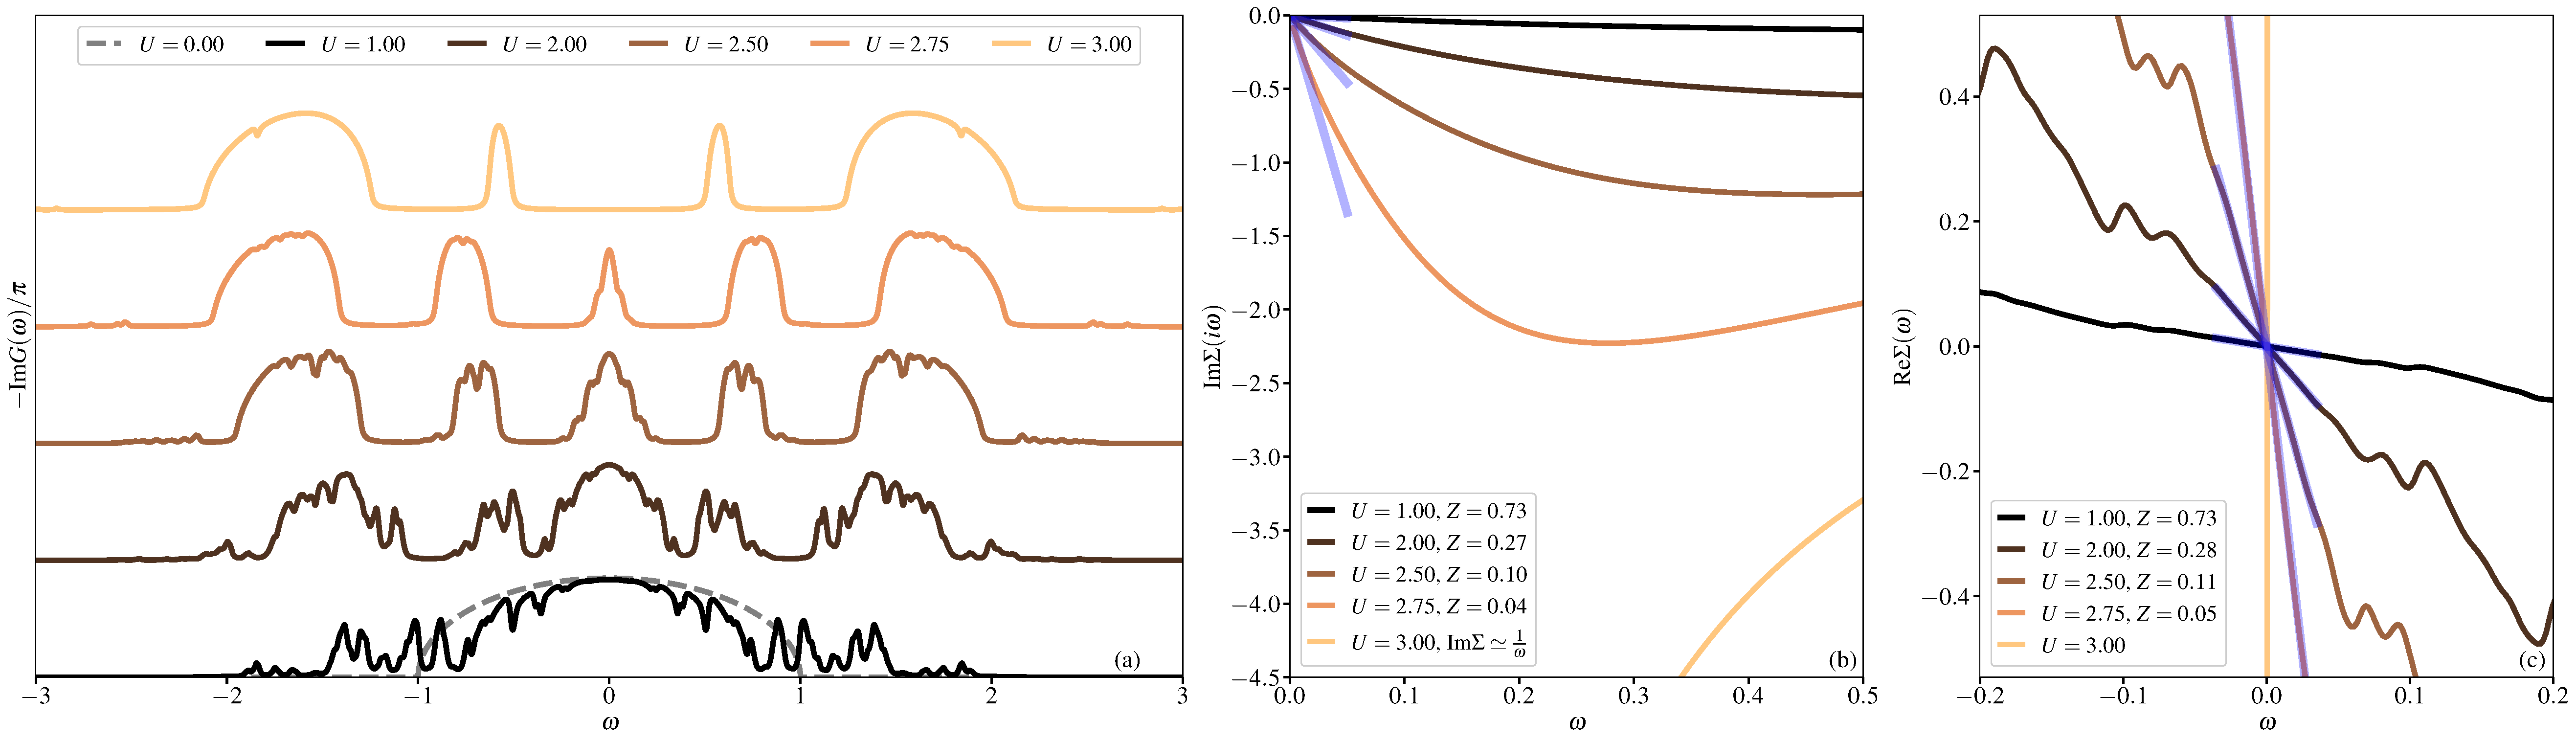
\includegraphics[width=\linewidth]{figures/figBethe.pdf}
    \caption{\label{figEx1}%
      \textbf{The metal-insulator Mott transition.}
      (a) Evolution of the spectral function $-\Im{G}(\omega)/\pi$ as
      a function of increasing interaction $U$. The critical
      interaction $U_\mathrm{c}\simeq 2.8D$ separates the correlated metal $U<U_\mathrm{c}$ from
      the Mott insulator $U>U_\mathrm{c}$.
      (b)-(c) The corresponding evolution of the Matsubara self-energy
      $\Im\Sigma(i\omega)$ (b) and
      real-axis one $\Re\Sigma(\omega)$ across the Mott
      transition. For a particle-hole symmetric case, both allow to
      estimate the renormalization constant $Z$ (see main text), using
      linear order expansion in frequency (blue solid lines). The
      values of $Z$ are reported in the legend.
      The Mott insulating solution is associated with a singularity at
      $\omega=0$ of $\Im\Sigma$.
    }
\end{figure}

The formation of a spectral gap separating the Hubbard bands in the 
Mott insulating phase is associated with the divergence of the 
imaginary part of the self-energy at the Fermi level. This divergence 
reflects the complete localization of the electrons, effectively 
suppressing coherent quasi-particle excitations. Causality dictates that the real part of the self-energy must also 
grow significantly near the singularity, making it impossible to 
satisfy the quasi-particle pole equation
$$
\omega+\mu-h^0-\e-\Re{\Sigma}(\omega)=0,
$$
which governs the formation of coherent excitations near the Fermi 
level.
Panels (B) and (C) illustrate this phenomenon by showing the evolution of the self-energy $\Sigma$. In panel (B), we present the Matsubara self-energy ${\rm Im}\Sigma(i\omega)$ in the low-energy regime. As the  interaction strength $U$ increases, this function progressively grows, eventually diverging as the critical interaction threshold $U > U_\mathrm{c}$ is crossed.
This divergence along the Matsubara axis is directly linked to the
particle-hole symmetry of the Bethe lattice, which pins the  ${\rm
  Im}\Sigma$ singularity at $\omega = 0$.
Panel (C) complements this picture by displaying the real part 
$\Re{\Sigma}(\omega)$ on the real-axis near the Fermi level. Here, increasing $U$ leads to a rapid rise of this component, culminating in a discontinuous behavior as the critical point is approached. This 
discontinuity directly reflects the divergence in the imaginary part
on the real-axis, confirming the transition to the Mott insulating state.


A quantitative measure of this transition is provided by the 
quasi-particle renormalization factor $Z$, which can be used to capture the degree of electron delocalization. This parameter ranges from 1 for a non-interacting metal to 0 for a fully localized Mott insulator. It is 
defined through the low-energy expansion of the self-energy as
$$
Z=\left(1-\frac{\partial\Re\Sigma}{\partial\omega}\Biggr|_{\omega\rightarrow
    0}\right)^{-1},
$$
which can also be estimated from the linear behavior of ${\rm Im}\Sigma(i\omega)$ for 
$\omega\to0$ in the metallic regime using the relation:
$$
   \frac{\Im\Sigma(i\omega_n)}{\omega_n}\Biggr|_{\omega_n\rightarrow 0}=
   \frac{1}{\pi}\int_{\mathbb R}d\epsilon \frac{\Re\Sigma(\epsilon)}{\epsilon^2}=
   \frac{\partial\Re\Sigma}{\partial\omega}\Biggr|_{\omega\rightarrow 0}.
$$

The linear fits highlighted in panels (B) and (C), along with the 
corresponding $Z$ values provided in the legends, clearly indicate that 
the slope of the self-energy at low energy increases with $U$ on both 
the Matsubara and real axes. At the transition point, this slope 
diverges, reflecting the onset of complete electron localization as 
$Z \to 0$, consistent with the singular behavior  
$-{\rm Im}\Sigma(\omega\to0) \to\infty$.






\subsubsection{Finite temperature (w2dynamics interface, CT-HYB benchmark)}\label{SecExamplesBetheDMFTW2D}
To demonstrate how the w2dynamics interface integrates with  \NAME, we briefly discuss how to solve the same problem, i.e. the Hubbard model on the Bethe lattice within DMFT using w2dynamics. 
In order to showcase the capabilities of \NAME to address low-temperature problems, we compare the continuous-time Quantum Monte Carlo (CTQMC) solver using the hybridization expansion method (CT-HYB) included in w2dynamics against the \NAME solver at finite temperature.  

Unlike \NAME, which provides only the impurity solver and bath optimization procedures and requires the user to implement the DMFT algorithm themselves (potentially using various methods), w2dynamics adopts a fundamentally different approach: a single Python script, {\tt DMFT.py}, handles the entire DMFT calculation, leveraging dedicated classes that implement the generic self-consistency. The w2dynamics calculation is then entirely controlled by a model-dependent parameters file {\tt Parameters.in}, which contains a number of variable specifications including options to control the ED solver inherited from \NAME. Further information about the functioning of w2dynamics can be found in Ref. \cite{Wallerberger2019CPC}           

Another important difference concerns the initial point of the iterative DMFT solution algorithm: while \NAME starts from a given discrete bath, w2dynamics is initialized with a zero self-energy function or alternatively reads this quantity from a converged solution file. Thus, when using the \NAME interface in w2dynamics, the initial Weiss field is determined using self-consistency and  an initial discrete bath is obtained through the \NAME bath optimization procedure. 

The following is the w2dynamics configuration file used to solve the Bethe lattice problem at finite temperature: 
\begin{lstlisting}[style=mybash,language={},numbers=none,basicstyle={\scriptsize\ttfamily}]
[General]
DOS             = Bethe           # support for the Bethe lattice is built-in
half-bandwidth  = 1               # list of half-bandwidths per orbital
NAt             = 1               # number of impurities
beta            = 100             # inverse temperature
mu              = 1.0             # chemical potential set to achieve half-filling
EPSN            = 0.0             # turns off filling-based chemical potential search
DMFTsteps       = 100             # given no convergence checking, we might want fewer
magnetism       = para            # symmetrize self-energies per spin
FileNamePrefix  = bethe_dmft_U2   # prefix for the output file name
fileold         = bethe_dmft*hdf5 # file to read an initial self-energy from
readold         = 0               # iteration number to read initial self-energy from, 0 turns off
mixing          = 0.5             # mixing, but mixes self-energies and not Weiss fields
mixing_strategy = linear          # linear mixing as in the Fortran example
FTType          = none            # (for CT-HYB): use the NFFT-measured G
solver          = EDIPACK         # use EDIpack as impurity solver, not default CTHYB

[Atoms]
[[1]]                             # one subsection per impurity
Nd              = 1               # number of orbitals
Hamiltonian     = Kanamori        # create a Hubbard-Kanamori interaction Hamiltonian
Udd             = 2.0             # equivalent to ULOC
Vdd             = 1.0             # equivalent to UST, meaningless for 1 orbital
Jdd             = 0.5             # equivalent to JH, JX and JP, also meaningless here

[EDIPACK]                         # further ED parameters, as in the Fortran example
NBATH           = 7               # number of bath sites
ED_TWIN         = True            # use twin symmetry
LFIT            = 2048            # number of Matsubara frequencies used for the bath fit
LANC_NGFITER    = 500             # number of Lanczos iterations for Green's function
CG_FTOL         = 1e-10           # conjugate-gradient tolerance
CG_NITER        = 2048            # maximum number of conjugate-gradient iterations
ED_FINITE_TEMP  = True            # at finite temperature T = 1/beta

[QMC]                             # Parameters for some grid sizes and the CT-HYB calculation
Ntau            = 1024            # imaginary time grid size
Niw             = 4096            # number of positive Matsubara frequencies
# parameters only relevant for CT-HYB follow
MeasGiw         = 1               # enable NFFT measurement of G
NCorr           = 175             # estimate of the autocorrelation length
Nmeas           = 200000          # number of measurements / sample size
Nwarmups        = 1000000         # number of initial warmup steps for Markov chain thermalization
\end{lstlisting}
Assuming the parameters are listed in a plain text file called 
{\tt bethe\_dmft.in}, the DMFT simulation can then by run on {\tt NC} cores via:
\begin{lstlisting}[style=mybash,numbers=none,morekeywords={mpiexec},deletekeywords={in}]
mpiexec -n NC /path/to/w2dynamics/DMFT.py bethe_dmft.in
\end{lstlisting}

The results are collected into an HDF5 \cite{The_HDF_Group_Hierarchical_Data_Format} archive in the usual w2dynamics format, including output quantities inherited from \NAME. Results can be viewed using the script {\tt hgrep} provided with w2dynamics or with other HDF5 tools. In this example we extract the Matsubara self-energy function $\Sigma(i\omega_n)$ for the last DMFT iteration:
\begin{lstlisting}[style=mybash,numbers=none]
/path/to/w2dynamics/hgrep latest siw-full -1
\end{lstlisting}

\begin{figure}%[t!]
  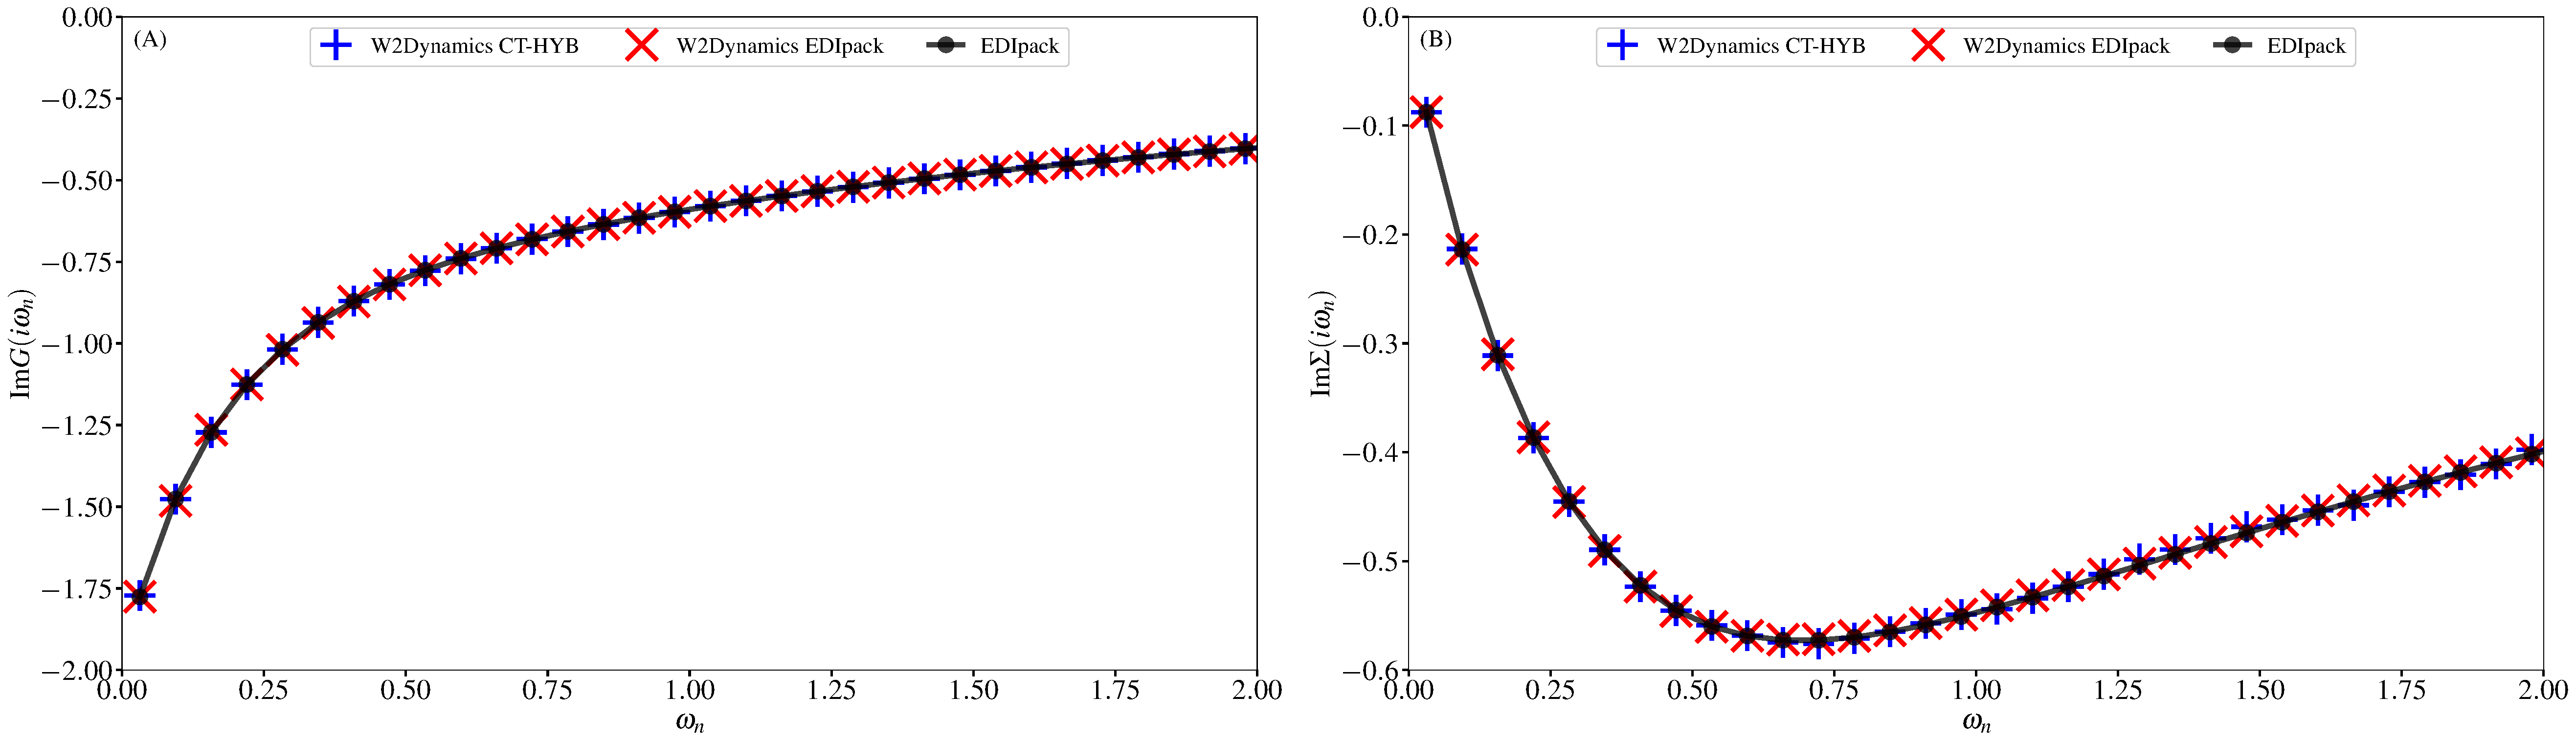
\includegraphics[width=\linewidth]{figures/figBetheW2D.pdf}
    \caption{\label{figEx1W}%
    \textbf{Finite temperature DMFT solution.}
    Comparison of the imaginary parts of the Green's function $\Im{G}(i\omega_n)$ and self-energy $\Im{\Sigma}(i\omega_n)$ from different solutions of the Hubbard model on the Bethe lattice using DMFT. Data are for $T/D=0.01$ and $U/D=2.0$. CTQMC results from the solver included with w2dynamics are compared against \NAME ED results, used both through the w2dynamics interface and with a standalone Fortran program. 
        }
\end{figure}

In \figu{figEx1W} we report a comparison of the results obtained using the hybridization expansion CTQMC and the \NAME ED method as solvers in w2dynamics. In addition we compare with results obtained using the Fortran API directly as shown in the previous subsection. Using DMFT, we solve the Hubbard model on a Bethe lattice for $T/D=0.01$ and $U/D=2.00$, corresponding to a correlated metallic state. 

In panel (A) we show the behavior of the imaginary part of the impurity Green's function $\Im{G}(i\omega_n)$ which is the direct output for both methods (note that w2dynamics does not directly have access to the real-axis Green's function when using the CTQMC solver). In panel (B) we show the same comparison for impurity self-energy $\Im{\Sigma}(i\omega_n)$. 
The results obtained from the three calculations are in excellent agreement with each other already for a small number of bath levels ({\tt NBATH=7}) and relatively low QMC statistics ({\tt Nmeas=200000} with {\tt NC=10} parallel processes).   



















\subsection{Attractive Hubbard model (Python API, {\tt ed\_mode=superc})}\label{SecExamplesAHM}
The second example we present concerns the DMFT description of the 
attractive Hubbard model \cite{Caffarel1994PRL,Toschi2005NJP,Toschi2005PRB} on a two-dimensional square lattice. 
This example has two main goals: (i) to demonstrate \NAME's support for $s$-wave superconductivity, and (ii) to showcase the Python API through a concrete example. 

The 
model Hamiltonian is given by:
$$
H = \sum_{\ka,\s} \epsilon(\ka) c^\dagger_{\ka\s} c_{\ka\s} 
    - U \sum_i n_{i\up} n_{i\dw},
$$
where $U > 0$, $c^\dagger_{i\s}$ 
is the creation operator for an electron at site $i$ with spin $\s$ and $c^\dagger_{\ka\s} = \tfrac{1}{\sqrt{N}} 
\sum_i e^{-i\ka \cdot R_i} c^\dagger_{i\s}$. 
The occupation operator is $n_{i\s} = c^\dagger_{i\s} c_{i\s}$, and 
the energy dispersion relation is $\e(\ka)=-2t[\cos{(k_x a)}+
\cos{(k_y a)}]$, where we set the lattice spacing 
$a=1$  and the choose the energy unit such that $4t=D=1$ for convenience.

The DMFT workflow for this case is largely similar to the previous 
example, but it now operates in the Nambu basis defined by the spinor $\psi_i=[\hat{c}_{i\up}\quad  \hat{c}^\dagger_{i\dw}]^T$ where the symbol $\hat{o}$ indicates the potential multi-orbital nature of the system, which reduces to a scalar in the present single-orbital case.
In this basis, the Green's function takes the matrix form:
\begin{equation}
  {\mathbf G} =
  \begin{pmatrix}
    \hat{G}_{\uparrow\uparrow} & \hat{F}_{\uparrow\downarrow}\\
    \hat{\bar{F}}_{\downarrow\uparrow}  &    \hat{\bar{G}}_{\downarrow\downarrow} \\
  \end{pmatrix}
\end{equation}
The components in the second row, denoted 
by $\hat{\bar{A}}$, are connected to the first row by particle-hole and time-reversal symmetries. The specific relations depend on the 
symmetry of the order parameter (here, $s$-wave) and whether the 
functions are defined on the Matsubara or real-frequency axis:
\begin{equation}
\begin{array}{cc}
  \hat{\bar{G}}(i\omega) = -\hat{G}^*(i\omega)\;; &  \hat{\bar{F}}(i\omega) = \hat{F}(i\omega)\\
  \hat{\bar{G}}(\omega)  = -\hat{G}^*(-\omega) \;; & \hat{\bar{F}}(\omega) = \hat{F}^*(i\omega)\\
\end{array}
\end{equation}  

The code implementation closely follows the structure of the previous 
example, with some notable adjustments related to the Nambu basis. 
These symmetries allow computing only the 
independent components in the first row, reducing 
the computational effort. 
Note that part of the operations required to implement the DMFT cycle are implemented in the Python module {\tt aux\_funx.py}, adapting from {\tt DMFTtools} functions.  
The initial part of the code handles the 
lattice structure and solver initialization, as described below.

\begin{lstlisting}[style=mypython,numbers=none,basicstyle={\scriptsize\ttfamily}]
import numpy as np
#Import EDIpack2py:
from edipack2py import global_env as ed
#Import MPI support 
import mpi4py
from mpi4py import MPI
#Import functions to build ${\color{comment-color}G_\mathrm{loc}}$ and perform DMFT self-consistency in Nambu space
from aux_funx import * 
import os,sys

#Start MPI framework:
comm = MPI.COMM_WORLD
rank = comm.Get_rank()
master = (rank==0)

#Functions: build 2D grid and dispersion ${\color{comment-color}\e(k)}$
def generate_kgrid(Nk):
    b1=2*np.pi*np.array([1.0,0.0])
    b2=2*np.pi*np.array([0.0,1.0])
    n1, n2 = np.meshgrid(np.arange(Nk), np.arange(Nk))
    n1=n1/Nk;n2=n2/Nk
    gridout = np.stack([n1.ravel(), n2.ravel()], axis=-1)
    return np.dot(gridout,[b1,b2])
    
def h_square2d(k,t):
  return -2*t*( np.cos(k[...,0,np.newaxis,np.newaxis])+
                np.cos(k[...,1,np.newaxis,np.newaxis]))*np.eye(ed.Norb)
    
#Read input
ed.read_input("inputAHM.conf")

#Generate ${\color{comment-color}H_k=\e(k)}$ and set Hloc
kgrid   = generate_kgrid(Nk)
Hk      = h_square2d(kgrid,t_hop)
Hloc    = np.sum(Hk,axis=0)/Nk**2
ed.set_hloc(Hloc.astype(complex))

#Build dispersion in Nambu space ${\color{comment-color}\e(k)\tau^z}$
HkNambu = np.array([h_square2d(kgrid,t_hop),-np.conj(h_square2d(-kgrid,t_hop))])

#Setup ED Solver
Nb=ed.get_bath_dimension()
bath = ed.init_solver()
\end{lstlisting}



The iterative scheme for the solution of DMFT closely follows the
sequence already discussed in \secu{SecExamplesBetheDMFT}:   
\begin{itemize}
\item[{\tiny {\bf EDIpack}}] Call the exact diagonalization {\bf impurity solver} {\tt
    ed.solve} providing the set of bath parameters $\vec{x}=\{V,h\}$  as input. 

\item[{\tiny {\bf EDIpack}}]  Use the dedicated
  input/output \NAME procedures to retrieve the self-energy functions  
  $\hat{\Sigma}(i\omega)$ and $\hat{S}(i\omega)$ on the 
  Matsubara axis.
  
\item[{\tiny {\bf EDIpack}}]
  Evaluate the interacting local Green's functions $\hat{G}_\mathrm{loc}$ and
  $\hat{F}_\mathrm{loc}$:
  \begin{equation}
  {\mathbf G}_\mathrm{loc}(i\omega) =
  \int_\RRR d\e \rho(\e)
  \begin{pmatrix}
    (i\omega +\mu)\hat{\11} - \hat{h}^0 - \hat{\Sigma}(i\omega) -\e & -\hat{S}(i\omega) \\
    -\hat{S}(i\omega) & (i\omega +\mu)\hat{\11} + \hat{h}^0 +
    \hat{\Sigma}^*(i\omega) +\e\\
  \end{pmatrix}^{-1}
\end{equation}

\item[{\tiny {\it User}}] Update the Weiss field's components, respectively 
  $\GG_0^{-1}$ and $\FF_0^{-1}$, through the {\bf self-con\-sis\-ten\-cy}
  relation: $\mathbfcal{G}^{-1}_0(i\omega) = {\mathbf G}^{-1}_\mathrm{loc}(i\omega) +
  {\mathbf \Sigma}(i\omega)$ in Nambu space.
  
\item[{\tiny {\it User}}\textgreater\ {\tiny {\bf EDIpack}}] Optimize the bath parameters $\vec{x}$ to best describe the updated
    Weiss fields, potentially using the \NAME provided conjugate gradient  fit
    procedures.
  \end{itemize}
%
The corresponding implementation in Python reads:
\begin{lstlisting}[style=mypython,numbers=none,basicstyle={\scriptsize\ttfamily}]
#DMFT CYCLE
converged=False;iloop=0
while (not converged and iloop<ed.Nloop):
    iloop=iloop+1
    #Solve quantum impurity problem for the current bath
    ed.solve(bath)    

    #Retrieve the Matsubara self-energy components ${\color{comment-color}\Sigma(i\omega_n) }$ and ${\color{comment-color}S(i\omega_n) }$
    Smats = np.array([ed.get_sigma(axis="m",typ="n"),ed.get_sigma(axis="m",typ="a")])   
    
    #Perform self-consistency levaraging {\tt aux\_funx.py} procedures:
    Gmats = get_gloc(wm*1j,ed.xmu,HkNambu,Smats,axis="m")
    Weiss = dmft_weiss_field(Gmats,Smats)    
    
    #Fit Weiss field and update the bath
    bath = ed.chi2_fitgf(Weiss[0],Weiss[1],bath)

    #Error check
    err,converged=ed.check_convergence(Weiss,ed.dmft_error)
ed.finalize_solver()
\end{lstlisting}


\begin{figure}[t!]
  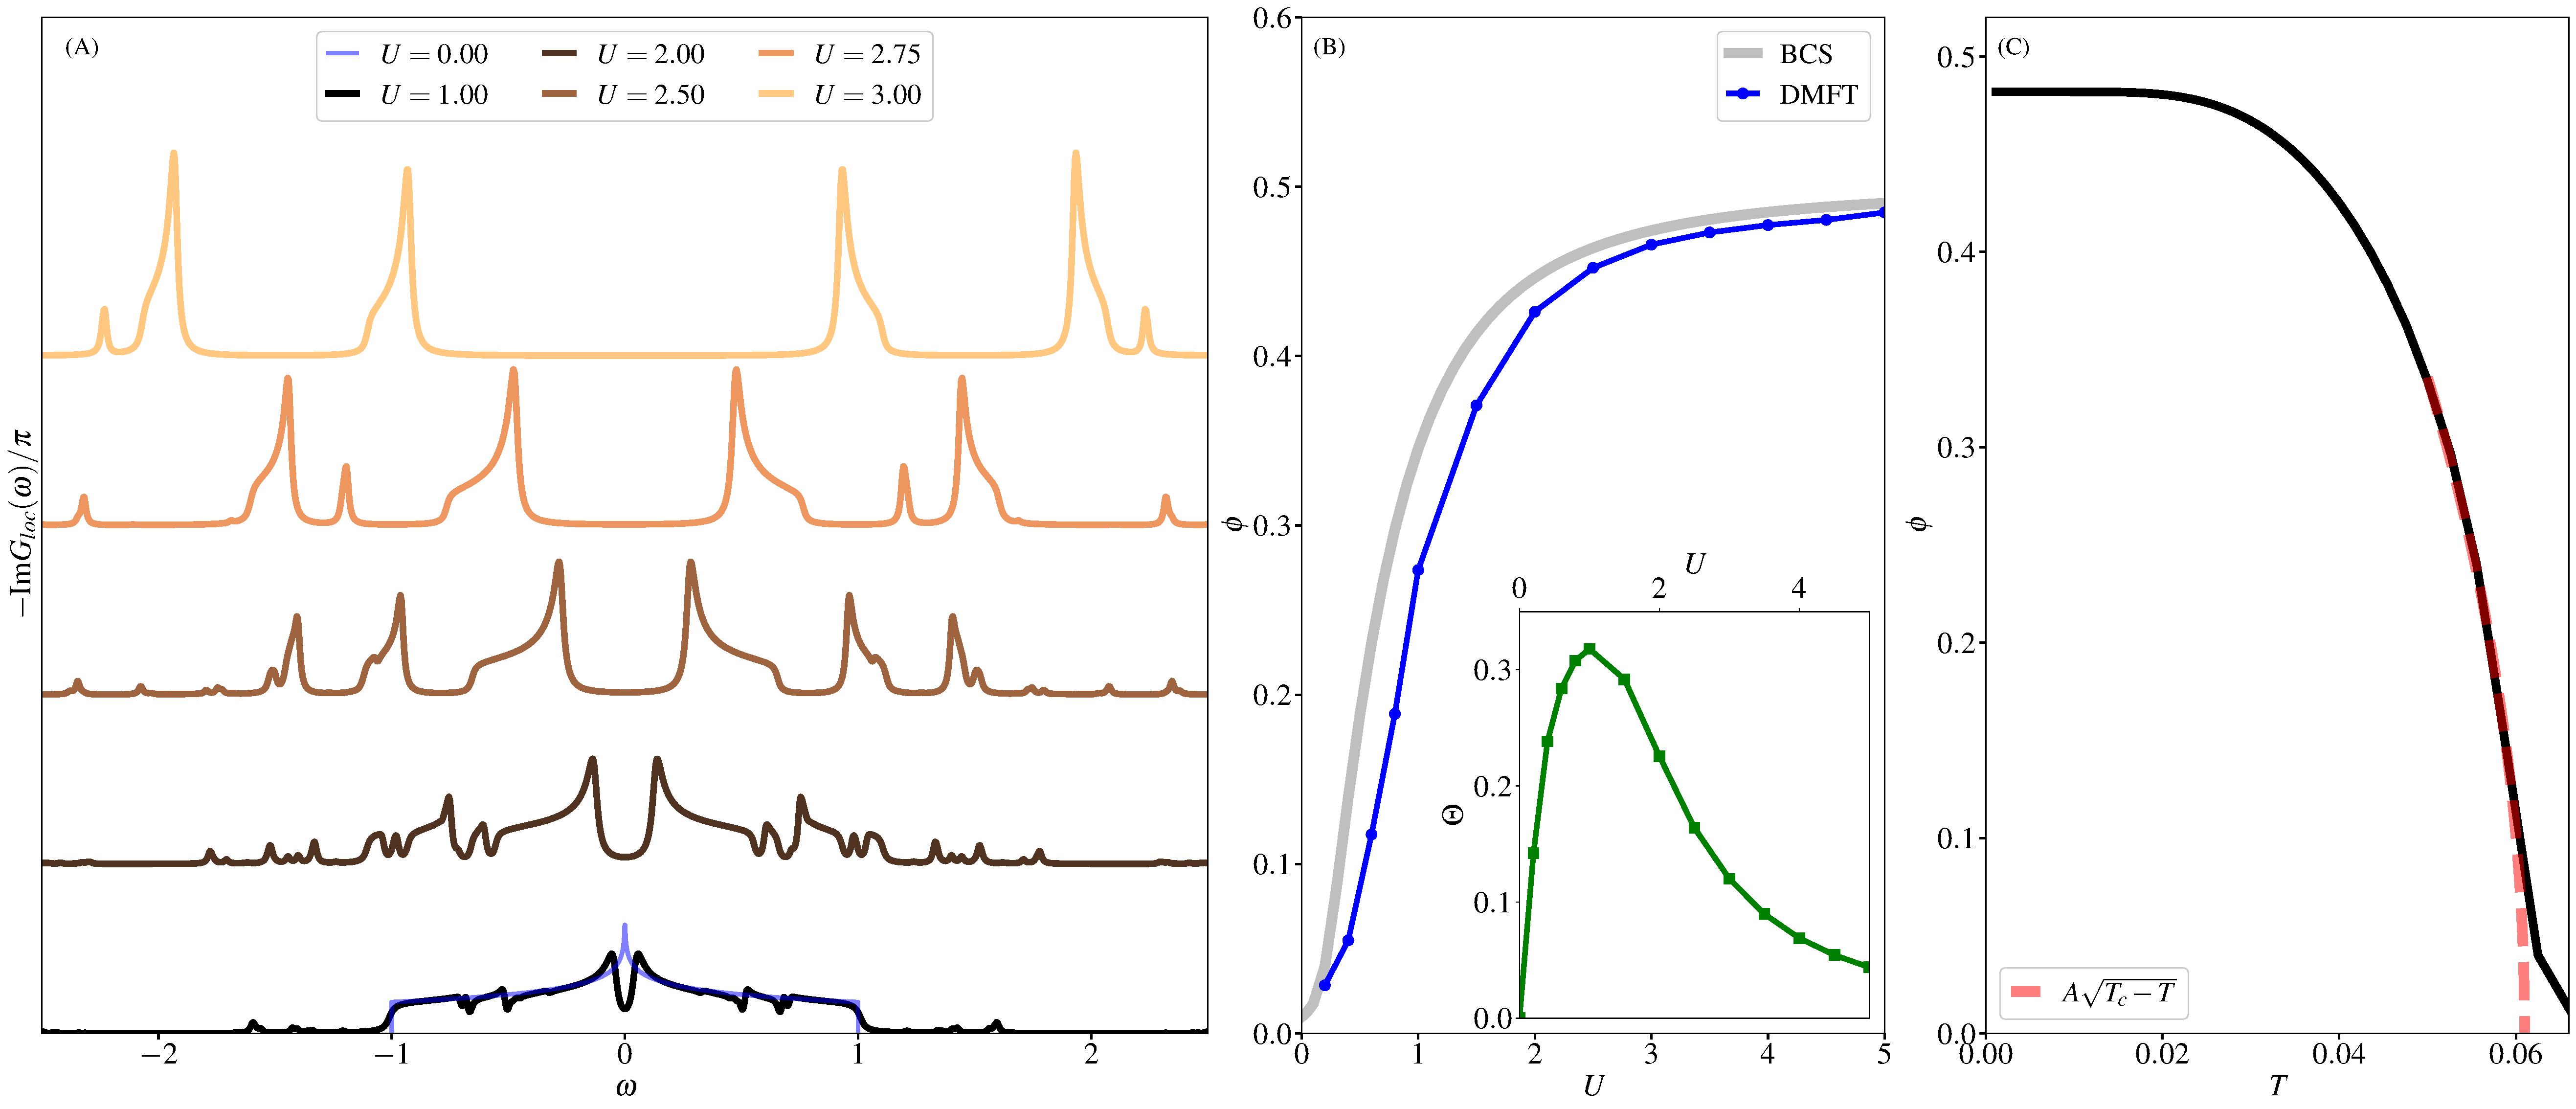
\includegraphics[width=\linewidth]{figures/figAHM.pdf}
    \caption{\label{figEx2}%
      \textbf{The BCS to BEC crossover.}
      (A) Evolution of the spectral functions
      $-\Im{G_\mathrm{loc}(\omega)}/\pi$ as a function of increasing
      attraction $U$. 
      (B) The order parameter $\phi=\langle c_\up c_\dw\rangle$ as a
      function of the attraction $U$. Data for BCS (gray) is compared
      to DMFT results (blue line and symbols). Inset: the correlation strength
      $\Theta$ (see main text) as a function of the
      attraction $U$ across the BCS-BEC crossover. 
      (C) Superconducting order
      parameter $\phi$ as a function of temperature across the
      superconductor-to-normal phase transition. Data for $U=4$. The
      fit highlights the critical behavior with a mean-field exponent
      $\beta=1/2$ (red dashed line) and parameters $A\simeq 3.7$, $T_\mathrm{c}=0.61$.       
        }
\end{figure}

\paragraph{Results.}
Here we showcase some results for the DMFT solution of the 
attractive Hubbard model across the BCS-to-BEC crossover regime \cite{Toschi2005PRB,Toschi2005NJP,Amaricci2014PRA} 
illustrating the capability of \NAME to handle $s$-wave 
superconductivity at both zero and finite temperatures.

To begin, panel (A) of \figu{figEx2} shows the evolution of the 
spectral density, obtained from the local normal Green's function as 
$-\tfrac{1}{\pi}\Im G_\mathrm{loc}(\omega)$, as a function of the 
attraction $U$. For any finite $U$, the Van Hove peak near the Fermi level characteristic of the 2D square lattice (visible at 
$U = 0$) is split by the formation of a superconducting gap. The latter reflects the emergence of a finite 
order parameter $\phi = \langle c_\up c_\dw \rangle$ and onset of superconducting coherence.

The evolution of the order parameter with attraction $U$ is presented in panel (B). The figure  
highlights the crossover from the weak-coupling BCS regime to the 
strong-coupling BEC regime. In the BCS limit, $\phi$ displays the 
characteristic exponential growth with $U$, known to be 
computationally challenging. In the opposite, strong-coupling, limit 
$\phi$ saturates at its theoretical maximum of $\phi \rightarrow 1/2$. The comparison with the BCS mean-field result 
(gray line) reveals the effect of local dynamical fluctuations, which  slightly suppress the order parameter, particularly in the intermediate regime. 
To further quantify these dynamical effects, we plot in the inset of the same panel the 
{\it correlation strength} \cite{Amaricci2015PRL,Amaricci2016PRB}
$\Theta=|S(i\omega\to 0)-S(i\omega\to\infty)|/S(i\omega\to\infty)$. 
Large values of $\Theta$ indicate an anomalous self-energy with 
significant dynamical effects, hence a more correlated superconducting state.
Our results show that the DMFT solution significantly departs from the BCS picture in the strongly correlated intermediate-coupling, a regime known to host the highest critical temperature \cite{Toschi2005NJP,Toschi2005PRB}.
% A different angle further illustrating the impact of dynamical fluctuations, is reported in panel (D). We show the evolution of the double occupancy $d = \langle n_\up n_\dw \rangle$ as a function of $U$ compared to the MF expression $d = 1/4 + \phi^2$. The DMFT 
% results obtained with \NAME show a slight increase in $d$ over the MF prediction in the BCS regime. As $U$ increases and local correlation becomes sizable, the double occupancy drops below 
% the MF result. 

Finally, we demonstrate the capability of \NAME to describe finite 
temperature effects. Panel (E) shows the temperature dependence of 
the order parameter $\phi(T)$ across the superconducting-to-normal 
transition. The mean-field nature of this transition is evident from 
the scaling near the critical temperature 
$\phi \sim (T_\mathrm{c} - T)^\beta$ with $\beta = 1/2$, consistent 
with  Ginzburg-Landau theory.

These results collectively illustrate the versatility of \NAME in 
handling both ground state and finite temperature superconducting 
phases, for instance capturing the complex physics of the BCS-BEC crossover with high accuracy.







\begin{figure}[ht!]
    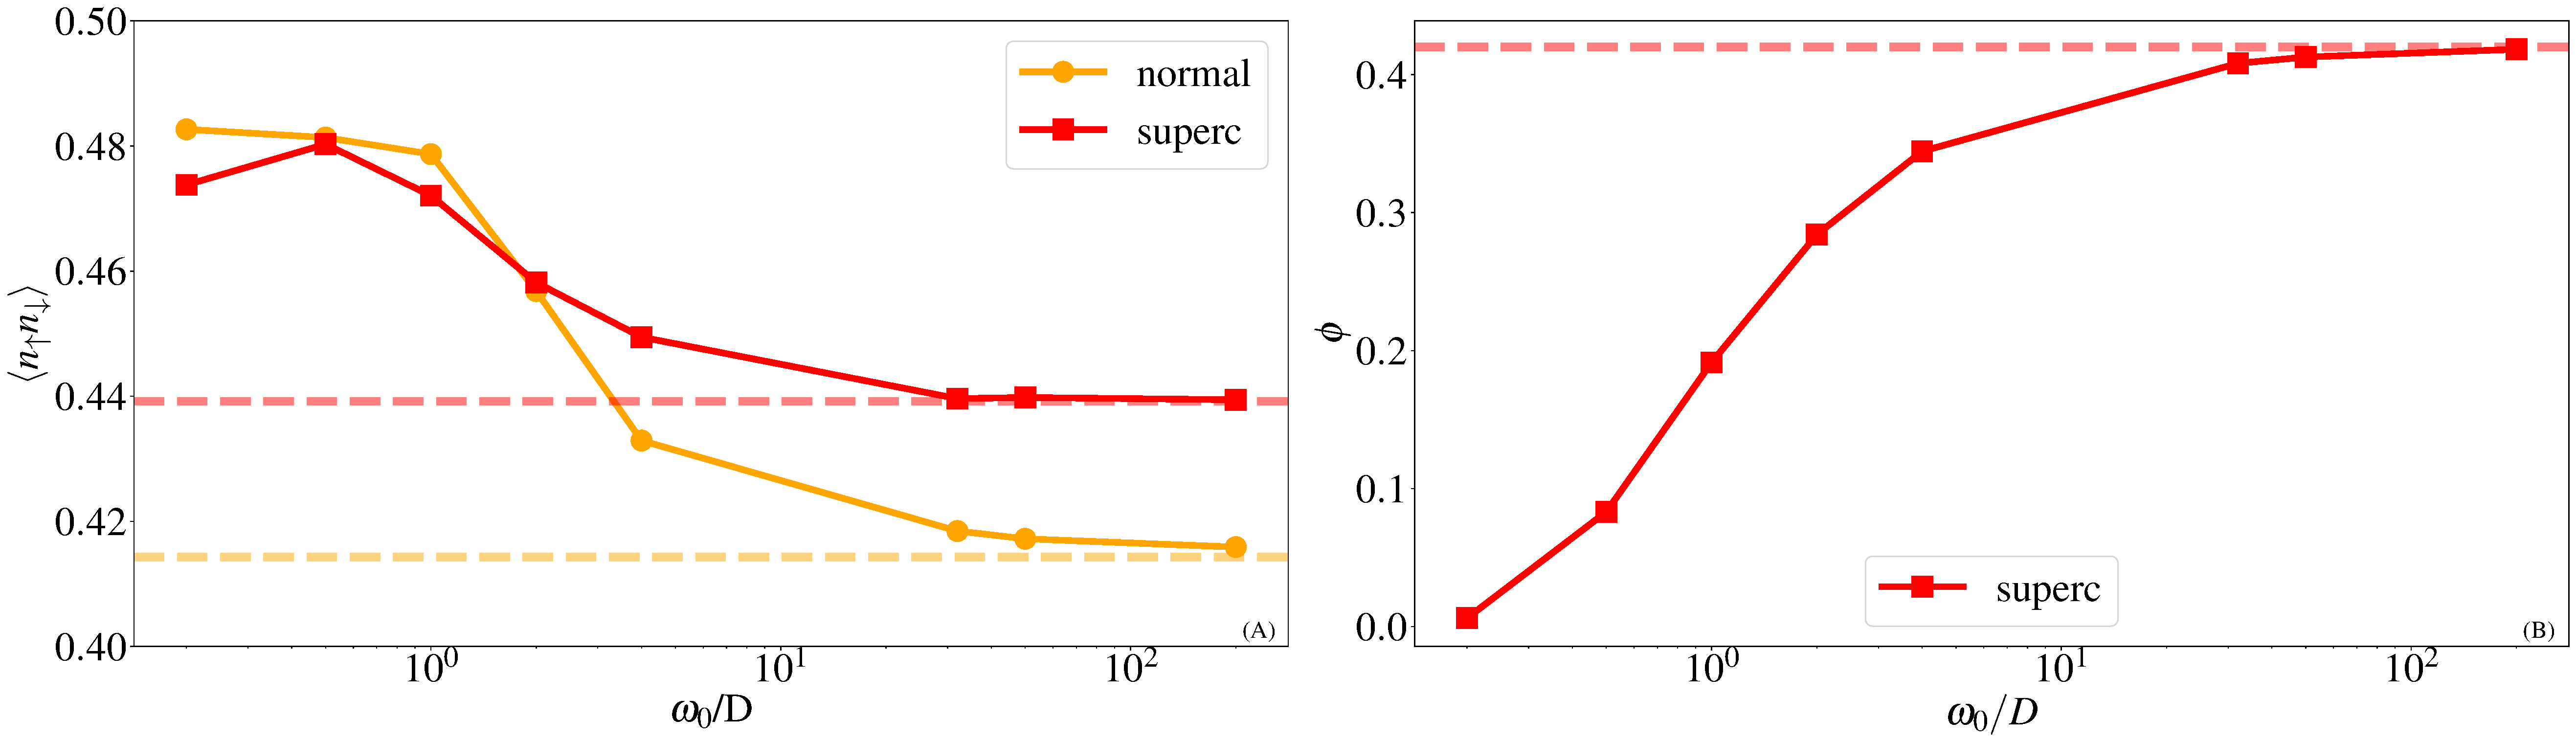
\includegraphics[width=\linewidth]{figures/figBethe_Holstein.pdf}
    \caption{\label{figEx5}
      Evolution of the double occupancy (A) and superconductive order parameter (B) as a function of $\omega_0/D$ for $\lambda=1$ in the normal (orange) and superconductive (red) phase. The horizontal broken lines are the values for the corresponding Hubbard model in the anti-adiabatic limit.}
\end{figure}


\subsection{Holstein model on the Bethe lattice (electron-phonon coupling)}

One of the new features introduced in \NAME is the support for local phonons in combination with superconductivity,
i.e. {\tt ed\_mode=superc}. In order to illustrate this property using a simple application, in this example we discuss the normal and
superconductive solution of the pure Holstein model on the Bethe lattice within DMFT.
Note that the code
implementation for this case is essentially identical to the listings in the previous sections
\ref{SecExamplesBetheDMFT} ({\tt ed\_mode=normal}) and
\ref{SecExamplesAHM} ({\tt ed\_mode=superc}), provided electron-electron interaction is set to zero and phonon parameters are properly configured.  

We consider the model introduced in \secu{SecExamplesBetheDMFT}
with $U=0$ and the additional phononic and electron-phonon terms:
\begin{equation} \label{eqex:H_Holstein}
    H_\mathrm{int} = \sum_i \Big[\omega_0 b^\dagger_i b_i + g(b^\dagger_i +
    b_i)\sum_{\sigma}\left(c^\dagger_{i\sigma}c_{i\sigma}
    -\frac{1}{2}\right)\Big]. 
\end{equation}
We focus on the half-filling regime of the particle-hole symmetric Bethe lattice DOS. We set the half-bandwidth as our energy unit $D=1$ and introduced the electron-phonon coupling $\lambda = \tfrac{2g^2}{\omega_0}$.  
The iterative DMFT solution algorithm follows the same principles illustrated in the previous sections. 

\paragraph{Results.}
In the following we discuss the adiabatic ($\omega_0\to0$) to
anti-adiabatic ($\omega_0\to\infty$) crossover for
the uniform solution of the Holstein model at constant coupling $\lambda=1.0$.
%
In the anti-adiabatic limit, the Holstein interaction takes a
particularly simple form:
\begin{equation}\label{HlikeAttraction}
    H_\mathrm{int} \overset{ \omega_0 \rightarrow \infty}{ \longrightarrow } -\frac{\lambda}{2} \sum_i \Big[\sum_\sigma\left(c^\dagger_{i\sigma}c_{i\sigma} -\frac{1}{2}\right) \Big]^2,
\end{equation}
which describes a local Hubbard-like attraction among electrons
(mediated by local phonons).
In the  adiabatic limit, $\omega_0 \rightarrow 0$ the system
enters a Bipolaronic Insulating phase for our
choice of the coupling \cite{Capone2006PRB}. 


We characterize the model solution by showing the evolution of the
double occupation $\langle n_{\up}n_{\dw}\rangle$ as a function of the
phonon frequency $\omega_0$, see panel (A) of \figu{figEx5}. In this panel we compare
the behavior for the normal phase ({\tt ed\_mode=normal}) and the superconductive
phase ({\tt ed\_mode=superc}). Our results capture the whole
crossover from adiabatic to anti-adiabatic regime. In the former
regime, the double occupation takes a similar value for the two
phases. However, approaching the anti-adiabatic regime, the two
solutions reach the limiting values corresponding to the residual
attraction \equ{HlikeAttraction}.   
To better characterize the nature of the superconducting
phase in the Holstein model, we report the evolution of the anomalous order
parameter $\phi$ in the adiabatic to anti-adiabatic crossover, see panel (B) of \figu{figEx5}.
The DMFT results obtained with \NAME show a rapid increase in the
superconducting order parameter as phonon frequency grows
large. Finally, in the anti-adiabatic regime, $\phi$ saturates to a
finite value corresponding to the attractive Hubbard-like interaction
of strength $\lambda/2$. 









\begin{figure}[t!]
    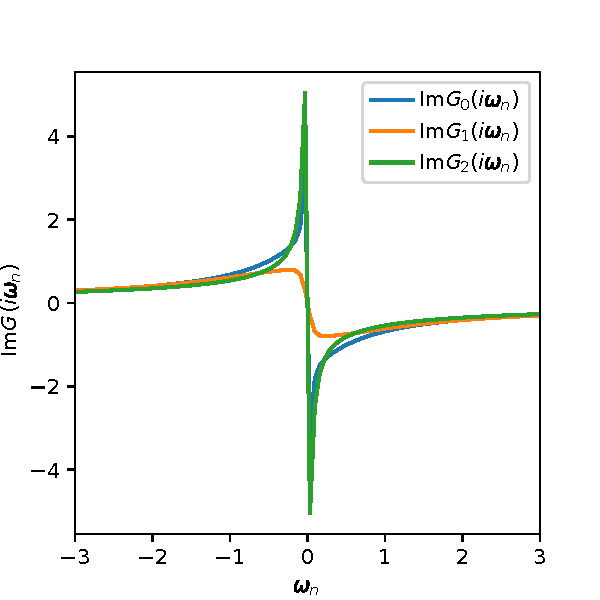
\includegraphics[width=0.5\linewidth]
        {figures/G_iw.pdf}
    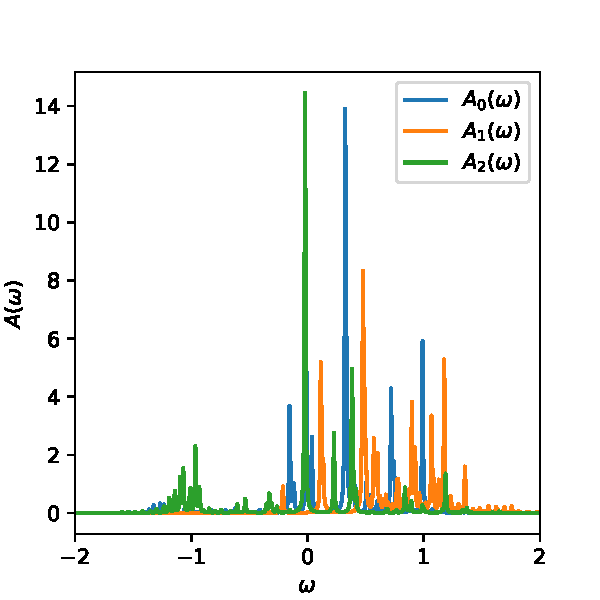
\includegraphics[width=0.5\linewidth]
        {figures/A_w.pdf}
    \caption{\label{figEx3}%
        Imaginary part of the Matsubara Green's function $G_\alpha(i\omega_n)$ (left) and the
        corresponding orbital-resolved spectral function $A_\alpha(\omega) = -\Im{G_\alpha(\omega)} / \pi$ (right) computed for a
        three-orbital impurity model with an interaction of the Hubbard-Kanamori
        type (\ref{Hint}). This illustration is produced by the EDIpack2TRIQS
        example script presented in \secu{SecExamplesTRIQS}.
    }
\end{figure}

\subsection{Multi-orbital impurity with Kanamori
  interaction (TRIQS interface)}
\label{SecExamplesTRIQS}

We proceed to demonstrate how to use the EDIpack2TRIQS compatibility
layer (\secu{sSecInteropTRIQS}) to solve a quantum system comprised by a
3-orbital correlated impurity coupled to a few non-interacting bath sites.
The interaction term of the impurity Hamiltonian is in the Hubbard-Kanamori
form of \equ{Hint}.

A Python script implementing a calculation that makes use of EDIpack2TRIQS
generally begins with a few module imports.
\lstinputlisting[style=mypython,
                 numbers=none,
                 basicstyle={\scriptsize\ttfamily},
                 firstline=1, lastline=13]
{figures/hubbard_kanamori.py}

One then proceeds to defining the system under consideration. In this case we
consider an impurity atom with three correlated orbitals and two bath states
per each impurity orbital, which corresponds to {\tt bath\_type=normal} in \NAME. This information must be encoded in the fundamental
set objects that are later used to construct the solver.
\lstinputlisting[style=mypython,
                 numbers=none,
                 basicstyle={\scriptsize\ttfamily},
                 firstline=15, lastline=26]
{figures/hubbard_kanamori.py}
The next step is to define a TRIQS many-body operator expression that represents
the Hamiltonian to be diagonalized.
\lstinputlisting[style=mypython,
                 numbers=none,
                 basicstyle={\scriptsize\ttfamily},
                 firstline=28, lastline=67]
{figures/hubbard_kanamori.py}
Finally, one creates a solver object and performs the actual calculation by
calling its method {\tt solve()}. This is normally the most time- and
memory-consuming step.
\lstinputlisting[style=mypython,
                 numbers=none,
                 basicstyle={\scriptsize\ttfamily},
                 firstline=69, lastline=83]
{figures/hubbard_kanamori.py}
The computation results are readily available as attributes of the solver
object. The following code snippet shows how to access measured expectation
values of the static observables, and how to employ the plotting framework of
TRIQS to visualize the obtained Matsubara and real-frequency impurity Green's
functions (\figu{figEx3}).
\lstinputlisting[style=mypython,
                 mathescape=false,
                 numbers=none,
                 basicstyle={\scriptsize\ttfamily},
                 firstline=85, lastline=113]
{figures/hubbard_kanamori.py}


















\subsection{Interacting Bernevig-Hughes-Zhang model (Fortran API, {\tt ed\_mode=nonsu2})}
In this section, we focus on the DMFT solution of the interacting
Bernevig-Hughes-Zhang (BHZ) model.
As shown in Ref. \cite{Amaricci2023PRB}, this model exhibits an excitonic phase at moderate
interactions in which opposite orbital electrons and holes across the band gap bind and form a coherent phase \cite{Knolle2017PRL,Jia2022NP,Varsano2020NN,Blason2020PRB,Amaricci2023PRB,Giuli2023PRB}

We consider a system of two-orbital electrons on a square
lattice, interacting via a Hubbard-Kanamori term. This system realizes a quantum spin Hall insulator \cite{Kane2005PRL,Bernevig2006S,Hasan2010RMP,Hohenadler2011PRL,Amaricci2015PRL,Tang2017NP,Amaricci2023PRB,Paoletti2024PRB}.
We consider a suitable matrix basis in terms of the Dirac
matrices $\Gamma_{a\a}=\sigma_a\otimes \tau_\a$, where $\sigma_a$ and
$\tau_\a$ are Pauli matrices, respectively, in the spin and orbital
pseudo-spin space. The  model Hamiltonian reads
$$
H = \sum_{k}\psi_{k}^\dagger H(k)\psi_{k} + H_{\rm int},
$$
where $\psi_{k}=[c_{1\uparrow k}, c_{2\uparrow k},
c_{1\downarrow k}, c_{2\downarrow k} ]^T$ is the spinor collecting
annihilation operator $c_{a\sigma k}$ destroying an electron at
orbital $a=1,2$ with spin  $\sigma=\up,\dw$ and lattice momentum
$k$. The non-interacting part of the Hamiltonian is:
$$
H(k) = \left[M-2t(\cos{k_x}+\cos{k_y}) \right]\Gamma_{03} +
   \lambda\sin{k_x}\Gamma_{31} -   \lambda\sin{k_y}\Gamma_{02},
$$
where $M$ is the mass term, which plays the role of a crystal
field splitting among the orbitals. The presence of this term breaks
the symmetry in the orbital pseudo-spin channel.
The  interaction reads: 
$$
   H_{\rm int} = (U-J)\frac{\hat{N}(\hat{N}-1)}{2} - J\left( \frac{1}{4}\hat{N}^2 +
   \hat{S_z}^2 - 2 \hat{T_z}^2\right),
 $$
 where $\hat{N}=\tfrac{1}{2}\psi_i^\dagger \Gamma_{00}\psi_i$ is the
total density operator,
$\hat{S_z}=\tfrac{1}{2}\psi_i^\dagger \Gamma_{30}\psi_i$ is the total
spin polarization operator and $\hat{T_z}=\tfrac{1}{2}\psi_i^\dagger
\Gamma_{03}\psi_i$ is the orbital pseudo-spin polarization operator.
This form corresponds to the density-density part of the
Kanamori interaction. We neglect the pair-hopping and spin-flip purely
for numerical reasons \cite{Amaricci2022CPC}. 
%
In the non-interacting regime this model describes a
quantum spin Hall insulator (QSHI) for $M<4t$ and a trivial Band
Insulator (BI) for $M>4t$.
The transition point at $M=4t$ describes the formation of a gapless Dirac state at  $k=[0,0]$.  


The code implementation follows the same guidelines discussed above for the other examples. The user is required to generate the Hamiltonian $H(k)$ on a discretized Brillouin zone. 
This is employed to evaluate the local interacting Green's function:
$$
G_\mathrm{loc}(z) = \tfrac{1}{N_k}\sum_k \left[z+\mu-H(k)-\Sigma(z)
\right]^{-1}, 
$$
entering in self-consistency conditions $\GG^{-1}=G_\mathrm{loc}^{-1}+\Sigma$. 
Here  $\z\in\CCC$, $N_k$ is the number of $k$-points   and $\Sigma(z)$ is the self-energy matrix  obtained from the DMFT solution of the problem.  
Moreover, the $H(k)$ is used to  construct the {\it renormalized} topological Hamiltonian \cite{Wang2010PRL,Wang2012PRX,Blason2023PRB}
$$
H_\mathrm{top} = \sqrt{Z}[H(k) + \Re\Sigma(\omega\to0)]\sqrt{Z}, 
$$
where $Z$ is the renormalization constant matrix. The matrix $H_\mathrm{top}$ describes the
low-energy properties of the many-body solution and can be used to characterize the topological nature of the interacting system \cite{Gurarie2011PRB,Wang2012PRX,Wagner2023NC,Blason2023PRB,Bau2024PRB}.  




\begin{figure}[t!]
  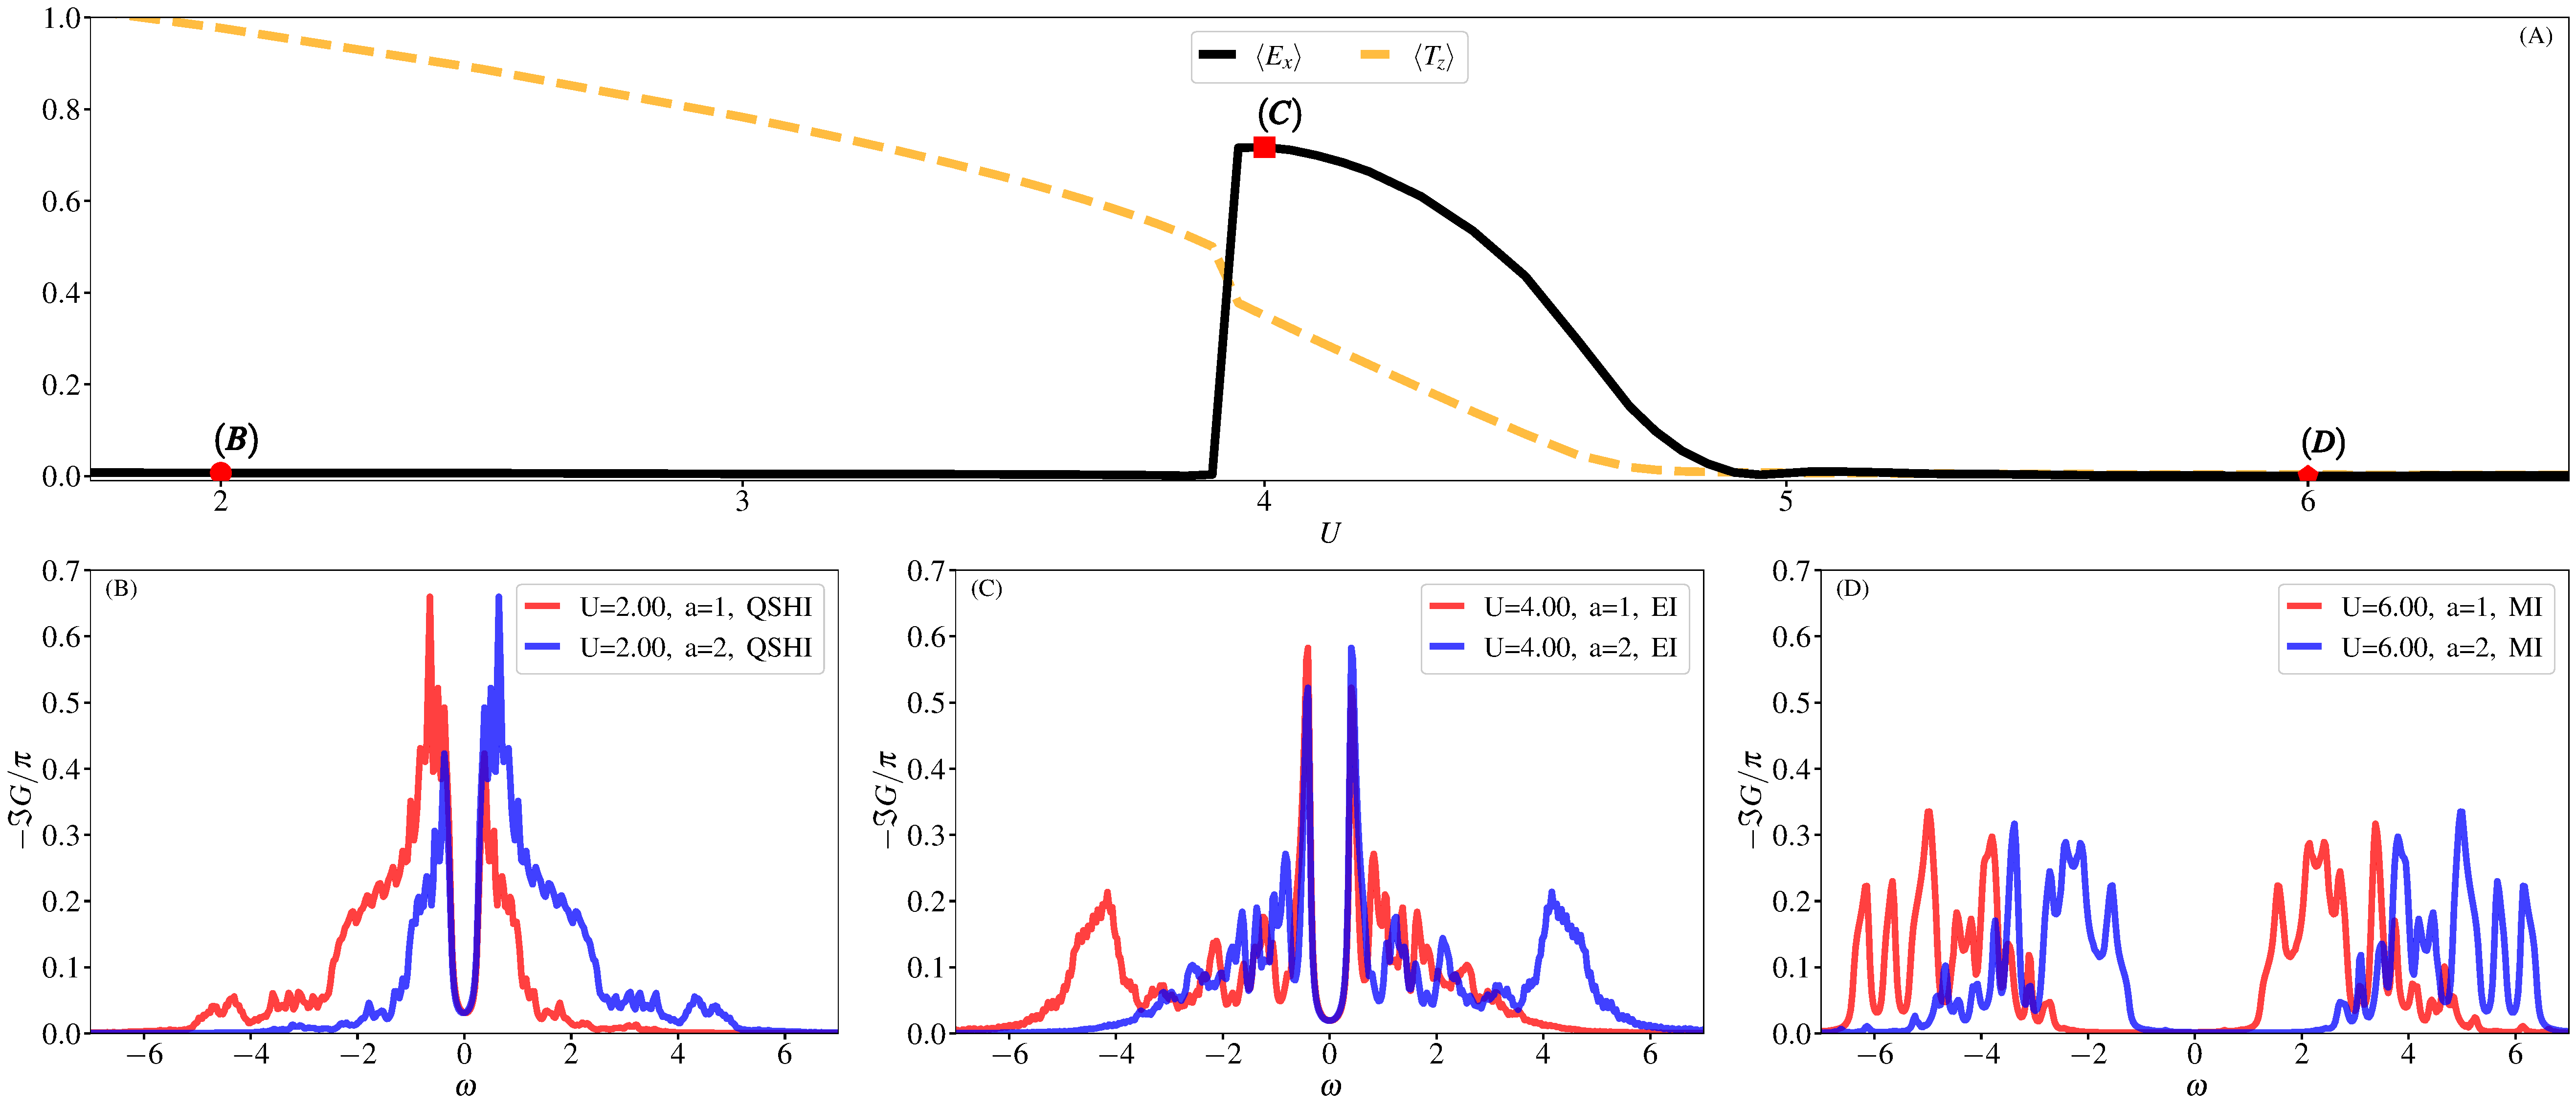
\includegraphics[width=\linewidth]{figures/figBHZ.pdf}
    \caption{\label{figEx4}%
      \textbf{Topological and Exciton Transition.}
      (A) Evolution of the spin-triplet,
      in-plane excitonic order parameter $\langle E_x\rangle$ (black solid line) and
      orbital polarization $\langle T_z\rangle$ (orange dashed line) as a function of the
      interaction $U$.
      (B-D) Spectral functions of the two orbital electrons for three
      values of the interaction $U=2.00$ (red circle), $4.00$ (red
      square) and $6.00$ (red diamond) capturing, respectively, the
      QSHI \textbf{\textit{(B)}}, the Excitonic Insulator \textbf{\textit{(C)}} and the Mott Insulator
      \textbf{\textit{(D)}}. 
    }
\end{figure}

\paragraph{Results}
To capture the possible symmetry breaking in any excitonic channel
driven by the local interaction, we consider the vector order
parameter
$\vec{E}=[E_0,E_x,E_y,E_z]$, where $E_a=\langle\psi^\dagger
\Gamma_{a1}\psi \rangle$ \cite{Budich2014PRL,Kunes2014PRB,Kaneko2015JOPCS,Kunes2015JOPCM,Knolle2017PRL,Guerci2019PRM,Geffroy2019PRL,Mazza2020PRL,De-Palo2023PRB}.

The first component $E_0$ describes the singlet excitonic state,
whereas the remaining ones correspond to the triplet states with
different spin orientation \cite{Blason2020PRB,Amaricci2023PRB}.   
The analysis of the strong-coupling regime as well as impurity
excitonic susceptibility available in \NAME suggest the possible
instability to an in-plane spin-triplet exciton phase, i.e. with $E_x$
and/or $E_y$ different from zero, see \cite{Amaricci2023PRB}.
Interestingly, this state breaks several symmetries including
time-reversal and spin SU(2), which protect the topological state.

Here we showcase the DMFT description of the excitonic phase in the interacting BHZ model as a way to
illustrate the \NAME ability to capture matter phases with lowered spin-symmetry ({\tt ed\_mode=nonsu2}) and the use of {\tt
  bath\_type=replica}.

The initial part of the code implementation is a simple generalization of the previously discussed cases. 
The next non-trivial steps are: i) construct the lattice Hamiltonian $H(k)$ and the corresponding local part $H_\mathrm{loc}$, which determines the impurity properties, and ii) construct a matrix basis representation for the replica bath. These two steps can be implemented as follows: 

\begin{lstlisting}[style=fstyle,numbers=none,basicstyle={\scriptsize\ttfamily}]
   !> Set $\smash{{\color{comment-color}H_\mathrm{loc}}}$ 
   allocate(Hloc(Nso,Nso))
   Hloc = sum(Hk,dim=3)/Lk
   where(abs(dreal(Hloc))<1d-6)Hloc=zero

   !EDIpack: set the impurity Hamiltonian: $\smash{{\color{comment-color}H_\mathrm{loc}\to h^0}}$
   call ed_set_hloc(Hloc)


   !EDIpack: set the replica bath matrix basis $\smash{{\color{comment-color}  \vec{\Gamma}}}$ and $\smash{{\color{comment-color}  \vec{\lambda}}}$
   !Here Nsym=4.
   !Build the basis and init the variational parameters:
   allocate(lambdasym_vector(Nbath,4))
   allocate(Hsym_basis(Nso,Nso,4))
   Hsym_basis(:,:,1)=Gamma03 ;lambdasym_vector(:,1)= Mh
   Hsym_basis(:,:,2)=Gamma01 ;lambdasym_vector(:,2)= sb_field
   Hsym_basis(:,:,3)=Gamma31 ;lambdasym_vector(:,3)= sb_field
   Hsym_basis(:,:,4)=Gamma11 ;lambdasym_vector(:,4)=-sb_field
   
   !EDIpack: set the basis and initial values of $\smash{{\color{comment-color}  \vec{\lambda}}}$
   call ed_set_Hreplica(Hsym_basis,lambdasym_vector)
   
   !EDIpack: get bath dimension and allocate user bath to this size
   Nb=ed_get_bath_dimension(4)
   allocate(Bath(Nb))
   
   !EDIpack: Initialize the ED solver
   call ed_init_solver(bath)
\end{lstlisting}
Here we use the local non-interacting Hamiltonian 
$H_\mathrm{loc}=\tfrac{1}{N_k}\sum_k H(k)$ to set 
$h^0_{\a\b\s\s'}$, i.e. the impurity Hamiltonian. To anticipate the
possibility of forming an excitonic ordered phase, the replica bath
is constructed out of a matrix basis with 4 distinct elements
$\Gamma_{03}$, $\Gamma_{01}$, $\Gamma_{31}$, $\Gamma_{11}$ which are proportional, respectively, to the mass term, the exciton singlet
$E_0$, the exciton triplet along easy-axis $E_z$ and in-plane
$E_x$ (we assume $E_y=0$ leveraging on residual $U(1)$ in-plane symmetry). 
In the following we consider the case of $M=1$, which corresponds to a QSHI in the non-interacting limit and $J/U=0.25$.
The implementation is nearly identical to the cases discussed above and
we report it here for completeness:
\begin{lstlisting}[style=fstyle,numbers=none,basicstyle={\scriptsize\ttfamily}]
   iloop=0;converged=.false.
   do while(.not.converged.AND.iloop<nloop)
     iloop=iloop+1
     
     !EDIpack: Solve the impurity problem
     call ed_solve(bath)

     !EDIpack: Retrieve ${\color{comment-color} \Sigma(i\omega)}$
     call ed_get_sigma(Smats,axis="mats")
     
     !Get $\color{comment-color}G_\mathrm{loc}$ using $\color{comment-color}\mathrm{DMFTtools}$
     call get_gloc(Hk,Gmats,Smats,axis="m")
     
     !Update the Weiss field (self-consistency) using $\color{comment-color}\mathrm{DMFTtools}$
     call dmft_self_consistency(Gmats,Smats,Weiss)

     !Linear mixing the Weiss fields
     if(iloop>1)Weiss = wmixing*Weiss + (1.d0-wmixing)*Weiss_;Weiss_=Weiss

     !EDIpack: Fit to update the bath
     call ed_chi2_fitgf(Weiss,bath,ispin=1)
     
     !Check convergence: using $\color{comment-color}\mathrm{DMFTtools}$
     converged = check_convergence(Weiss(1,1,:),dmft_error,nsuccess,nloop)
   enddo  
 \end{lstlisting}
 
%
The main effect of the interaction on the topological properties is contained in the mass term renormalization.  
The real part of the self-energy being proportional to $\Gamma_{03}$
corrects the mass term with respect to its bare value: $M_\mathrm{eff}=M+\tfrac{1}{4}\Tr{\Re\Sigma(i\omega\to0)}$. 
To leading order (mean-field) this correction is proportional to $\tfrac{U-5J}{4}\langle
\hat{T}_z\rangle$. So, for our choice of parameters, the effect of
interaction would be to effectively reduce the mass term. Thus, in the strong-coupling limit the two orbitals get populated by one electron per site, reaching the
conditions for the formation of a Mott insulating state.
This effect is highlighted in panel (A) of \figu{figEx4}, where we report the progressive reduction of the
orbital polarization  $\langle T_z\rangle$ and, thus, of the effective mass. 


In the same panel (A), we show that at intermediate coupling 
the DMFT solution features the formation of a
region of exciton condensation with $\langle E_x\rangle>0$, $\langle
E_0\rangle=\langle E_z\rangle=0$. 

Unlike the static mean-field description \cite{Blason2020PRB}, the
transition from the QSHI topological state to the Excitonic Insulator 
(EI) becomes of first-order upon including the local dynamical fluctuations \cite{Paoletti2024PRB,BellomiaKMH} contained in DMFT. 
The EI continuously evolves into a Mott Insulator (MI)
for larger interaction (neglecting for simplicity any 
antiferromagnetic ordering that would naturally occur in this
regime).
The \NAME solution of this model nicely captures the two transitions which involve breaking of the spin symmetry group SU(2). 



To further illustrate the nature of the three distinct phases of this
system, we rely on the direct access to the real-axis spectral
function provided by \NAME solver. In panels (B)-(D) of \figu{figEx4}
we report the spectral functions $-\Im{G}_{a\up,\mathrm{loc}}(\omega)/\pi$ for
$a=1,2$, and three distinct values of the interaction
$U$ placing the solution, respectively, in the QSHI, the EI and the MI.

The correlated QSHI is characterized by the presence of an 
inverted band gap featuring a substantial orbital spectral mixing. The
EI spectrum is instead characterized by a narrow gap, related to the
finite order parameter, flanked by two sharp resonances and featuring
larger high-energy weight.
Finally, in the MI the two-orbital spectral function describes the two 
characteristic Hubbard bands separated by a large Mott gap.  








\subsection{Interacting Kane-Mele model (Fortran API, EDIpack2ineq, iRDM)}

To complete the overview of \NAME's features, we consider an additional interacting quantum spin-Hall insulator model, defined on the honeycomb lattice, with two inequivalent sites in the unit cell. Neglecting the Rashba spin-orbit interaction and discarding any ionic character of the unit cell, the noninteracting Kane-Mele Hamiltonian \cite{Kane2005PRLa,Kane2005PRL} can be written in momentum space as
\begin{align*}
    H_\mathrm{KM} = \sum_{{k}} \psi^\dagger_{{k}} H({k}) \psi_{{k}},
\end{align*}
with $\psi_{{k}} = [c_{{k},\mathrm{A},\up},\,c_{{k},\mathrm{B},\up},\,c_{{k},\mathrm{A},\dw},\,c_{{k},\mathrm{B},\dw}]$ and
    \begin{align}
    H({k}) 
    &= x_{{k}}\Gamma_{01} + y_{{k}}\Gamma_{02} + \delta_{{k}}\Gamma_{33}, \label{eq:Hk_kanemele}\\[1mm]
   x_{{k}}&=t\bigl[\cos({k}\cdot{u})+\cos({k}\cdot{v})+1\bigr],\nonumber\\
   y_{{k}}&=t\bigl[\sin({k}\cdot{u})+\sin({k}\cdot{v})\bigr],\nonumber \\
   \delta_{{k}}&=2\lambda_\mathrm{so}\bigl[\sin({k}\cdot{u})-\sin({k}\cdot{v}) - \sin({k}\cdot{u} -{k}\cdot{v})\bigr], \nonumber
\end{align}
where ${u} = (3a/2, \sqrt{3}a/2)$, and ${v} = (3a/2, -\sqrt{3}a/2)$ 
are suitable basis vectors for the honeycomb lattice, $t$ is the
nearest-neighbor hopping amplitude and $\lambda_\mathrm{so}$ is 
the amplitude of a complex next-nearest-neighbor hopping,
with a spin-dependent $\pm\tfrac{\pi}{2}$ chiral phase arising from spin-orbit coupling, which is well-known to open a topological gap at the Fermi level \cite{Kane2005PRLa,Kane2005PRL}.
The spinorial $4\times4$ matrices $\Gamma_{a\ell} = \sigma_a\otimes\tau_\ell$ are 
defined in terms of Pauli matrices $\sigma_a$, $\tau_\ell$ referred, respectively 
to spin and sublattice degrees of freedom.
% , with the convention that 
% $\sigma_0$ and $\tau_0$ are $2\times2$ identity matrices.
To investigate the effects of electron-electron repulsion we consider a local Hubbard term \cite{Hohenadler2013ROPIP,Rachel2018ROPIP}:
\begin{equation}
    H_\mathrm{KMH}  = H_\mathrm{KM} 
    + U\sum_{i}\Biggl[
                        \left(n_{i,\up} - \frac{1}{2}\right)
                        \left(n_{i,\dw} - \frac{1}{2}\right)
                      \Biggr],
    \label{eq:KMHmodel}
\end{equation}
where $n_{i,\sigma}=c^\dagger_{i,\sigma}c_{i,\sigma}$ are the 
local spin-density operators. The interaction is written in an explicitly 
particle-hole symmetric form so that the model is at half-filling for zero
chemical potential.

The essential features of the ground state phase diagram have been established by intensive multi-method analyses \cite{Rachel2018ROPIP}.
For $\lambda_\mathrm{so}=0$ the model describes a Dirac semimetal, up to large repulsion, and magnetizes to an isotropic Néel state above a critical $U/t$ ratio \cite{Sorella1992ELE,Castro-Neto2009RMP}.
% \footnote{In contrast to the expectations for a generic half-filled bipartite lattice, for which the ground state is antiferromagnetic for any nonzero interaction, this property descends from the peculiar properties of Dirac cones: the vanishing density of states at the Fermi level renders the logarithmic instability ineffective, even in the presence of perfect nesting \cite{Sorella1992ELE,Castro-Neto2009RMP}.}.
For a finite spin-orbit coupling $\lambda_\mathrm{so}\neq0$, the quantum spin-Hall state results increasingly stable against magnetic ordering, due to its symmetry-protected nontrivial topology. Furthermore, the long-range ordering
eventually stabilized at large $U/t$, is characterized by a lowered
spin symmetry, due to the inherent coupling of spin and lattice
degrees of freedom that favors in-plane easy-axis magnetization \cite{Griset2012PRB}, as predicted by Hartree-Fock and $t$-$J$ perturbative expansions \cite{Rachel2010PRB} and
later confirmed by Auxiliary-Field Quantum Monte Carlo (AFQMC) 
simulations \cite{Hohenadler2013ROPIP}.

To treat the in-plane Néel ordering with \NAME, we can once again
exploit the \texttt{ed\_mode=nonsu2} option, allowing off-diagonal 
spin amplitudes in all dynamical matrices and so eventually in the
resulting impurity self-energy.
Referring to the two inequivalent sublattices as
A and B, whereas a standard off-plane ($S_z$)
calculation would enforce Néel symmetry (AFM$_\perp$)  as
$\Sigma^\mathrm{A}_{\up\up} = \Sigma^\mathrm{B}_{\dw\dw}$, 
$\Sigma^\mathrm{A}_{\dw\dw} = \Sigma^\mathrm{B}_{\up\up}$,
with
$\Sigma^\mathrm{A}_{\up\dw} = \Sigma^\mathrm{A}_{\dw\up} = \Sigma^\mathrm{B}_{\up\dw} = \Sigma^\mathrm{B}_{\dw\up} = 0$,
an in-plane magnetization (AFM$_\parallel$) corresponds to
$\Sigma^\mathrm{A}_{\up\up} = \Sigma^\mathrm{B}_{\up\up}$, 
$\Sigma^\mathrm{A}_{\dw\dw} = \Sigma^\mathrm{B}_{\dw\dw}$,
$\Sigma^\mathrm{A}_{\up\dw} = -\Sigma^\mathrm{B}_{\dw\up}$, 
$\Sigma^\mathrm{A}_{\dw\up} = -\Sigma^\mathrm{B}_{\up\dw}$.

The same off-diagonal spin symmetry must be realized also in
the bath Hamiltonian, which can be conveniently achieved with
either the \texttt{replica} and \texttt{general} choices for 
the \texttt{bath\_type} option. The most robust strategy to
verify that the ground state of the model is magnetized in the
plane also in DMFT is to allow either an $S_z$ or an $S_x$ (equivalently $S_y$) magnetization in the bath, and then
compare the energies of the respective solutions at $T=0$. 
The corresponding Hamiltonian forms are:
\begin{align}
    H^\mathrm{bath}_\perp &= 
        \sum_{p=1}^{N_\mathrm{b}}(\epsilon_p \sigma_0 + m_p \sigma_z), 
        \label{eq:afmz_dmft_ansatz} \\[1mm]
    H^\mathrm{bath}_\parallel &= 
        \sum_{p=1}^{N_\mathrm{b}}(\epsilon_p \sigma_0 + m_p \sigma_x).
        \label{eq:afmx_dmft_ansatz}
\end{align}
which corresponds to $N_\mathrm{sym}=2$, with
$\lambda_{1,p} \equiv \epsilon_p$ as the degenerate
bath levels that are Zeeman split by $\lambda_{2,p} \equiv m_p$, respectively in the $S_z$ and $S_x$ bases 
(see \secu{sSecBath}).

\begin{lstlisting}[style=fstyle,numbers=none,basicstyle={\scriptsize\ttfamily}]
program dmft_kane_mele_hubbard
  !Load EDIpack library 
  USE EDIPACK
  !Load the inequivalent impurities extension
  USE EDIPACK2INEQ
  ...
  !Setup bath and solver for anisotropic AFM phases
  !> define the symmetry-basis:
  Nineq = 2
  Nsym = 2
  allocate(Hsym_basis(Nspin*Norb,Nspin*Norb,Nsym))
  Hsym_basis(:,:,1) = pauli_0
  select case(ansatz)
    case('off-plane');Hsym_basis(:,:,2) = pauli_z
    case('in-plane') ;Hsym_basis(:,:,2) = pauli_x
  end select
  !> initialize the symmetry parameters
  allocate(lambdasym_vectors(Nineq,Nbath,Nsym))
  call build_replica_band(onsite_band,ed_hw_bath,Nbath)
  ! (user-built guess of the starting bath levels)
  lambdasym_vectors(:,:,1) = onsite_band 
  lambdasym_vectors(:,:,2) = 0d0 ! paramagnetic
  !> define a symmetry-breaking AFM kick, to help numerics
  if(afmkick)then
     lambdasym_vectors(1,:,2) = +sb_field
     lambdasym_vectors(2,:,2) = -sb_field
  endif
  !> setup H_bath inside the solver
  select case(bath_type)
    case('replica')
        call ed_set_Hreplica(Hsym_basis,lambdasym_vectors)
    case('general')
        call ed_set_Hgeneral(Hsym_basis,lambdasym_vectors)
  end select
  !> finally initialize the two solver instances, one per sublattice
  !  (the EDIpack2ineq layer automatically dispatches it for the two
  !   impurity models, if we feed a Bath with the [Nineq,Nb] shape!)
  Nb = ed_get_bath_dimension(Hsym_basis)
  allocate(Bath(Nineq,Nb))
  call ed_init_solver(Bath)
  ... 
\end{lstlisting}

The DMFT loop can then be implemented, with the explicit solution of two
independent impurity problems (prone to numerical noise) or by solving
only one impurity problem and building the full solution by exploiting 
the appropriate Néel symmetry:

\begin{lstlisting}[style=fstyle,numbers=none,basicstyle={\scriptsize\ttfamily}]
   iloop=0;converged=.false.
   do while(.not.converged.AND.iloop<nloop)
      iloop=iloop+1
      !
      !> Solve the two inequivalent impurity problems
      if(neelsym)then
        !> solve just one sublattice and get the other by Neel symmetry
        call ed_solve(Bath(1,:))
        call ed_get_sigma(Smats(1,:,:,:,:,:),axis='m')
        select case(ansatz)
            case('off-plane')
             Smats(2,2,2,:,:,:) = Smats(1,1,1,:,:,:) 
             Smats(2,1,1,:,:,:) = Smats(1,2,2,:,:,:) 
             if(master)write(*,*) ">>> Enforcing AFMz symmetry"
            case('in-plane')
             Smats(2,1,1,:,:,:) = Smats(1,1,1,:,:,:)   
             Smats(2,2,2,:,:,:) = Smats(1,2,2,:,:,:)   
             Smats(2,1,2,:,:,:) = -Smats(1,1,2,:,:,:)  
             Smats(2,2,1,:,:,:) = -Smats(1,2,1,:,:,:) 
             if(master)write(*,*) ">>> Enforcing AFMx symmetry"
        end select
      else
         !> solve both sublattices independently using EDIpack2ineq:
         !  mpi_lanc=T => MPI lanczos, mpi_lanc=F => MPI for ineq sites
         call ed_solve(Bath,mpi_lanc=.true.)
         !> retrieve all self-energies:
         call ed_get_sigma(Smats,Nineq,axis='m')
         !
      endif
      !
      !> Get ${\color{comment-color}G_{loc}(i\omega_n) }$ : using ${\color{comment-color}\mathrm{DMFTtools}}$
      call dmft_gloc_matsubara(Hk,Gmats,Smats)
      !
      !> Update local Weiss fields $\smash{{\color{comment-color}\GG^{-1}_0 = G^{-1}_{loc} + \Sigma}}$: using ${\color{comment-color}\mathrm{DMFTtools}}$
      call dmft_self_consistency(Gmats,Smats,Weiss)
      !
      !> Fit the new bath:
      !  - normal mode: normal/AFMz and we fit spin-components independently
      !  - nonsu2 mode: broken Sz-conservation and we fit
      !                 both spin components together
      select case(ed_mode)
       case("normal")
         call ed_chi2_fitgf(Bath,Weiss,ispin=1)
         call ed_chi2_fitgf(Bath,Weiss,ispin=2)
       case("nonsu2")
         call ed_chi2_fitgf(Bath,Weiss,Hloc)
      end select
      !
      !> linear mixing and convergence check: using ${\color{comment-color}\mathrm{DMFTtools}}$
      if(iloop>1) Bath = wmixing*Bath + (1.d0-wmixing)*Bath_prev
      Bath_prev = Bath
      converged = check_convergence(Weiss(:,1,1,1,1,:),dmft_error,nsuccess,nloop)
      !
   enddo
   !
   !> Compute Kinetic Energy: using ${\color{comment-color}\mathrm{DMFTtools}}$
   call dmft_kinetic_energy(Hk,Smats)
\end{lstlisting}

After convergence is reached, we evaluate some quantities of interest, e.g. computing the 
lattice kinetic energy (as implemented in the {DMFTtools} 
library). The potential energy, as well as the AFM order parameters
and impurity observables are automatically computed by \NAME, 
and saved to files with the appropriate inequivalent-impurity label.

We evaluate the total energy of both the AFM$_\perp$
and AFM$_\parallel$ calculations and compare them to establish which  is favored as the ground state of the system. In \figu{fig:KMenergy}(a)
we show results for the energy difference $E_\parallel-E_\perp$ across a wide range of $U/t$ and $\lambda_\mathrm{so}$ values. To assess the
degree of accuracy of our total energy calculation, we report in
\figu{fig:KMenergy}(b) a $\lambda_\mathrm{so}=0$ benchmark against
Hartree-Fock (simple static mean-field, but inherently variational), 
DMFT with NRG solver and lattice AFQMC data, as taken from 
Ref. \cite{Raczkowski2020PRB}. 

\begin{figure}
\hspace{1cm} (a) \hspace{6.5cm} (b)\\
    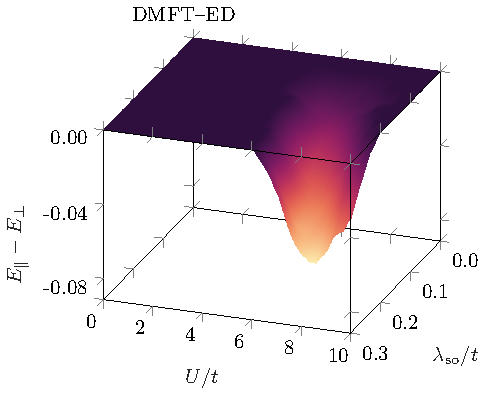
\includegraphics[width=0.47\linewidth,trim={0 0 0 5mm},clip]{figures/KMH_energy.pdf}\hfill
    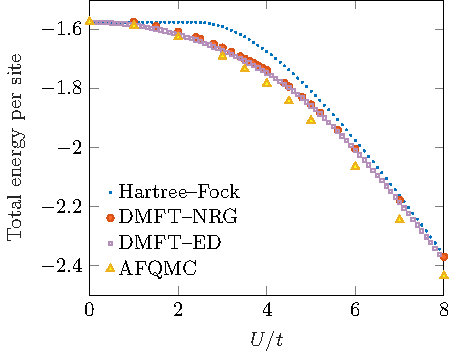
\includegraphics[width=0.45\linewidth]{figures/benchEnergy_honey.pdf}\\
    \caption{In panel (a) we report the total energy difference between 
    the in-plane and the
    off-plane AFM solutions found with \NAME at $T=0$. Negative values
    signal a ground state with in-plane magnetization. The plateau at zero
    energy difference marks the topological phase of the model (a 
    paramagnetic quantum spin-Hall insulator), at all points except on the $\lambda_\mathrm{so}=0$ line, where the ground state is an interacting
    Dirac liquid, at weak coupling, or an isotropic antiferromagnet at strong coupling. In panel (b) we compare the total energies, across the 
    $\lambda_\mathrm{so}=0$ line, to published data for Hartree-Fock,
    DMFT-NRG and AFQMC solutions \cite{Raczkowski2020PRB}.}
    \label{fig:KMenergy}
\end{figure}






\begin{figure}
    \centering
    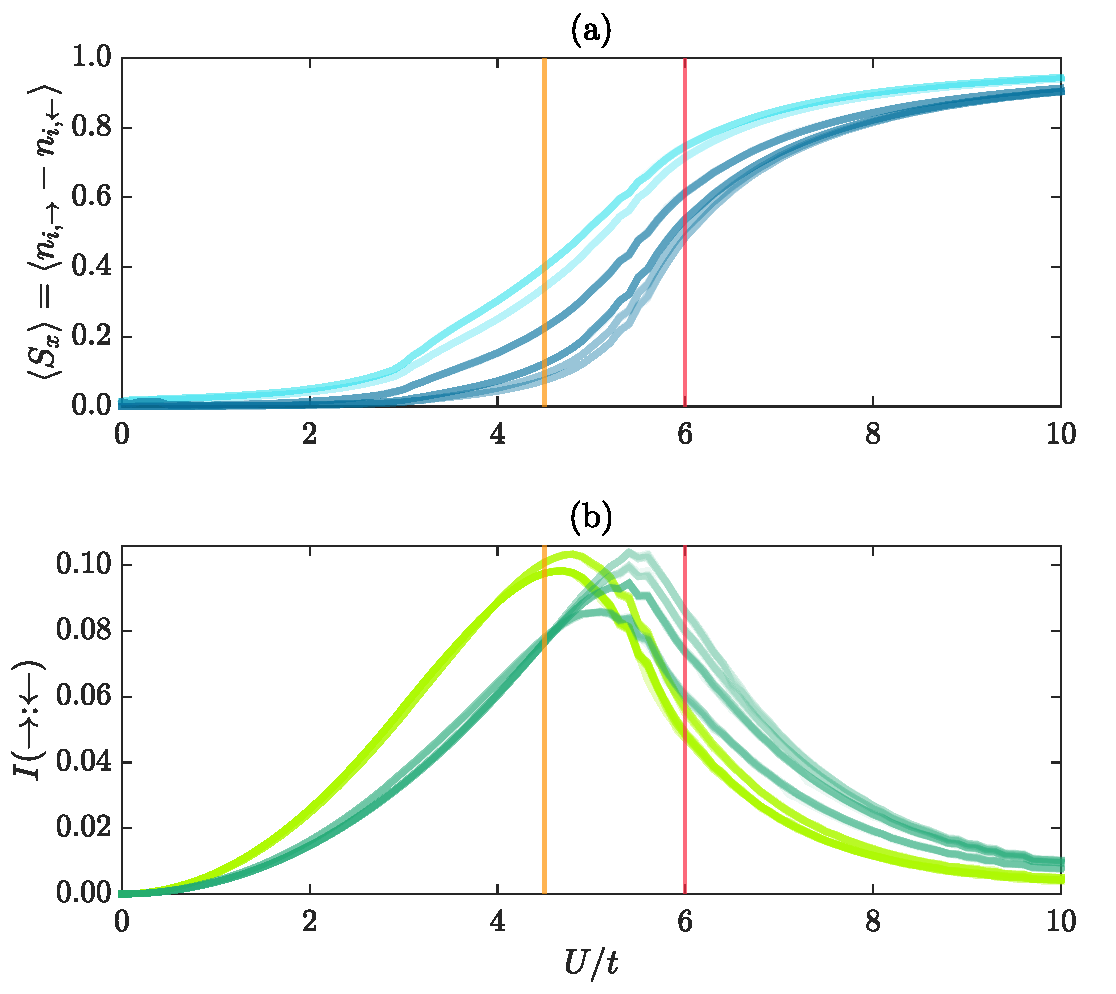
\includegraphics[width=0.8\linewidth]{figures/flakes_edipack.pdf}\\[1mm]
    (c) \hspace{10cm} (d) \\
    \hspace{1.2cm}
    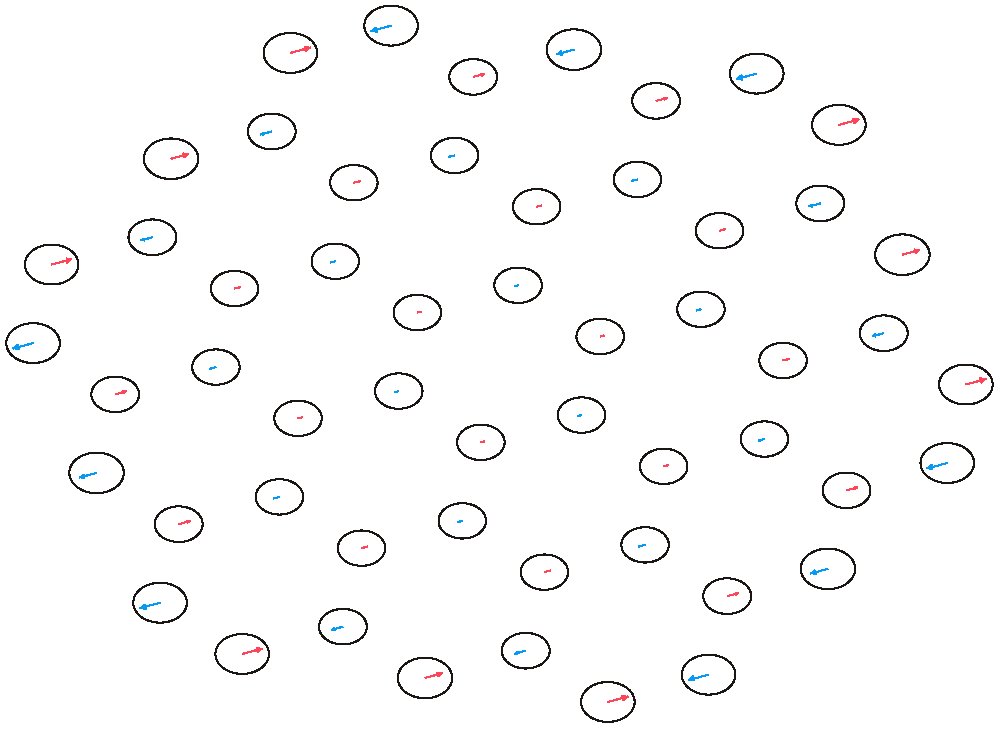
\includegraphics[width=0.33\linewidth]{figures/3NflakeU4.5_x.pdf} \hspace{1.2cm}
    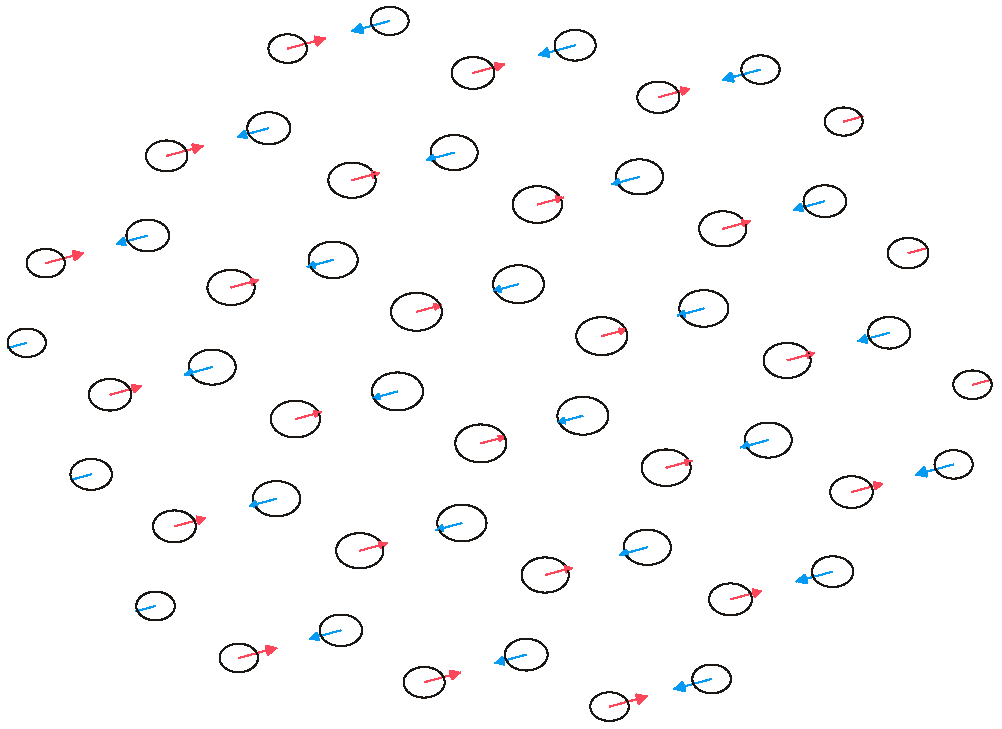
\includegraphics[width=0.33\linewidth]{figures/3NflakeU6_x.pdf} \vspace{3mm}
    \caption{Kane-Mele-Hubbard model at the nanoscale.
    In (a) the local in-plane
    magnetization $\ibra S_x \iket = \ibra n_{i,\rightarrow}-n_{i,\leftarrow}\iket$. In
    (b) the local correlation as measured by the mutual 
    information between local in-plane spin eigenstates
    $I(\rightarrow:\leftarrow)$ \cite{BellomiaPhD,BellomiaKMH,Bellomia_intracorr}. 
    Both the (a) and (b) panels mark the edge and ``bulk'' 
    sites in lighter and darker colors, respectively.
    In (c) and (d) a visual representation of the given 
    nano-system at different values of $U/t$, as marked 
    respectively by the orange and red vertical lines 
    in panels (a) and (b). The area of the 
    circles is proportional to $I(\rightarrow:\leftarrow)$, 
    the length of the arrows to $\ibra S_x \iket$.
    All data are taken at $\lambda_\mathrm{so}=0.3t$ and $T=0$.}
    \label{fig:KMflake}
\end{figure}


\subsubsection{Kane-Mele-Hubbard model at the nanoscale}
The capabilities of the EDIpack2ineq layer go well beyond the
simple case of a two-site unit cell. Building on the previous example, we can readily adapt the calculation to deal with a nanoscopic \cite{Amaricci2014PRA} system with $N_\mathrm{ineq}$ inequivalent atoms, such as hexagonal flakes
\cite{Valli2016PRB,Valli2018NL}.
We consider a 
$N_\mathrm{ineq}\times N_\mathrm{ineq}$ local Hamiltonian 
$H_\mathrm{loc}$ with open boundary conditions, and implementing
the self-consistent equations with a trivial single momentum 
$k=0$. In this configuration the system develops an inhomogeneous magnetization, so that in general no particular lattice symmetry group, e.g. N\'eel, can be exploited. 
% Some lowered point symmetry can be found, but a 
% safer approach of solving all the $N_\mathrm{ineq}$ impurity models
% leads to good results, with fair control of spatial numerical noise.

In \figu{fig:KMflake} we report results for a nanosystem of 
$N_\mathrm{ineq}=54$ sites, solved with the bath parametrization 
described in \equ{eq:afmx_dmft_ansatz}, for the in-plane 
antiferromagnetic state.
Panel (a) shows the interaction dependence of the local magnetization,
computed from the impurity ground state as  
$ \ibra S_x \iket = \ibra c^\dagger_{i,\up} c_{i,\dw} + c^\dagger_{i,\dw} c_{i,\up} \iket \equiv \ibra n_{i,\rightarrow} \iket - \ibra n_{i,\leftarrow} \iket$,
so that we can define the $S_x$ spin occupation numbers as
\begin{equation*}
    \ibra n_{i,\rightarrow} \iket \equiv \frac{\ibra n_{i,\up} + n_{i,\dw} \iket +
    \ibra c^\dagger_{i,\up} c_{i,\dw} + c^\dagger_{i,\dw} c_{i,\up} \iket}{2},
    \qquad
    \ibra n_{i,\leftarrow} \iket \equiv \frac{\ibra n_{i,\up} + n_{i,\dw} \iket -
    \ibra c^\dagger_{i,\up} c_{i,\dw} + c^\dagger_{i,\dw} c_{i,\up} \iket}{2},
\end{equation*}
which trivially satisfy the conservation of the local average charge $\ibra n_{i,\rightarrow} + n_{i,\leftarrow} \iket = \ibra n_{i,\up} + n_{i,\dw} \iket$.
Having a direct expression for $\ibra n_{i,\rightarrow} \iket$ and $\ibra n_{i,\leftarrow} \iket$
we can verify that the impurity reduced density matrix, computed by 
tracing the bath states in the \texttt{ed\_mode=nonsu2} representation 
(see \ref{sSecRDM}), once diagonalized, takes the familiar form
\cite{Zanardi2002PRA,Su2013MPLB,Walsh2019PRL} 
\begin{equation}
    \rho^\mathrm{imp} = 
     \begin{pmatrix}
            \left\ibra\left(1-n_{i,\rightarrow}\right)\left(1-n_{i,\leftarrow}\right)\right\iket   &    0          &       0       &   0 \\
                    0       &    \left\ibra n_{i,\rightarrow}\left(1-n_{i,\leftarrow}\right)\right\iket  &       0       &   0 \\
                   0       &       0   &    \left\ibra\left(1-n_{i,\rightarrow}\right)n_{i,\leftarrow}\right\iket      &   0 \\
                    0       &       0   &       0          &    \left\ibra n_{i,\rightarrow} n_{i,\leftarrow}\right\iket
        \end{pmatrix} 
\end{equation}
in the basis of the {\it natural} spin-orbitals
\cite{BellomiaPhD,BellomiaKMH,Bellomia_intracorr}, 
whose occupation numbers
are given by $n_{i,\rightarrow}$ and $n_{i,\leftarrow}$.
As  discussed in \cite{BellomiaPhD,BellomiaKMH,Bellomia_intracorr},
by defining the spin traces of $\rho^\mathrm{imp}$, as
\begin{equation}
    \rho^\mathrm{imp}_\sigma = 
    \Tr_{\bar{\sigma}} \left[\rho^\mathrm{imp}\right] =
    \begin{pmatrix}
        \ibra n_{i,\sigma} \iket & 0 \\
        0 & \ibra n_{i,\bar{\sigma}} \iket
    \end{pmatrix}
\end{equation}
we can directly measure local correlations by defining the mutual information
between the impurity spin-orbitals
$I(\rightarrow:\leftarrow) = 
    S(\rho^\mathrm{imp}_{\rightarrow}) + 
    S(\rho^\mathrm{imp}_{\leftarrow}) -
    S(\rho^\mathrm{imp})$,
where $S(\cdot)$ denotes the von Neumann entropy of its argument.

In panel (b) of \figu{fig:KMflake} we report the spatially resolved
interaction dependency of $I(\rightarrow:\leftarrow)$, as a direct 
observation of the enhanced local correlations at the boundary of the
finite system. While it is usually assumed that edge sites must be
more correlated than internal (``bulk'') sites, based on the reduced
lattice coordination, the inter-spin mutual information quantifies directly the phenomenon: the edge correlations,
marked in lighter green, are decidedly higher as long as the system 
remains in a weakly magnetized regime. When the local magnetization
exceeds half of its saturation value, all local correlations start to decrease,
as spin fluctuations are damped by ordering. Significantly, the edge 
correlations get lower than the bulk correlations as the maximum is 
crossed, consistently with the observation that their magnetization
is always higher and so their fluctuations are frozen faster.
Finally, we observe that the nanosystem of \figu{fig:KMflake} has 
finite local magnetization for arbitrary low interaction strengths,
in striking contrast with the infinite lattice. This is a well-known
effect of quantum confinement, as proposed in early works on graphene
flakes \cite{Valli2016PRB,Valli2018NL}.



%% References with bibTeX database:
\ifSubfilesClassLoaded{
  \bibliography{references}
}{}
\end{document}
